%!TEX TS-program = xelatex
%!TEX encoding = UTF-8 Unicode

% nobib: Don't load natbib with the tufte-book class, since we use biblatex instead.
\documentclass[justified,nobib]{tufte-book}
\morefloats
\usepackage{lgrind}
\usepackage{graphicx}
\usepackage{booktabs}
\usepackage{multirow}
\usepackage{moreverb}
\usepackage{alltt}
\usepackage{url}
\usepackage{array}
\usepackage{pdfpages}
\usepackage{wrapfig}
\usepackage{geometry}
\usepackage{enumitem}
\setkeys{Gin}{width=\linewidth,totalheight=\textheight,keepaspectratio}
\usepackage{fancyvrb}

% Use biblatex to allow for customization of citation vs. bibliography styles
% and use of \autocite puts the citation in the margin for Tufte classes.
% See also:
% - http://tex.stackexchange.com/questions/45934/can-i-use-biblatex-with-tufte-classes
% - http://tex.stackexchange.com/questions/12806/guidelines-for-customizing-biblatex-styles
\usepackage[
  firstinits=true,
  citestyle=authortitle-ibid,
  bibstyle=authoryear,
  autocite=footnote,
  citetracker=true,
  citereset=chapter,
  backend=bibtex,
  isbn=false,
  url=false
]{biblatex}
\addbibresource{/Users/powerpak/share/library.bib}
% Add a command to do a sidenote citation but with an adjustable Y offset.
\newcommand{\sidecite}[2][]{\ifthenelse{\equal{#1}{}}{\autocite{#2}}{\sidenote[][#1]{\cite{#2}}}}

% Further hacks to the biblatex style. (1) get rid of "In:" in the bibliography
\renewbibmacro{in:}{}
% Display all names (not just the first) in last-first order
\DeclareNameAlias{sortname}{last-first}

\usepackage{xpatch}
% Patch the citation formatting macros for authortitle-ibid to include a year.
% Also, if the citation was already seen in the same chapter, no need to repeat the title.
\xpatchbibmacro{cite}{\usebibmacro{cite:title}}{
  \addspace%
  \ifciteseen{\mkbibparens{\printtext[bibhyperref]{\printdate}}}{%
    \mkbibparens{\printdate}%
    \addcomma\addspace%
    \usebibmacro{cite:title}}}{}{}
\xpatchbibmacro{cite}{\setunit{\nametitledelim}}{}{}{}

% When citing something in-text (usually in a caption) just use author-year.
\xpatchbibmacro{textcite}
  {\usebibmacro{cite:title}}
  {\addspace\printtext[bibhyperref]{\printdate}}
  {}
  {}

% Customize link colors. These are standard dvips or svgnames color names.
% More colors at https://en.wikibooks.org/wiki/LaTeX/Colors#The_68_standard_colors_known_to_dvips
%   and http://www.latextemplates.com/svgnames-colors
\definecolor{AccentColor}{RGB}{0,77,128} % used for the title page
\hypersetup{%
  colorlinks = true,
  citecolor = Maroon,
  linkcolor = Maroon,
  urlcolor = Maroon
}

% XeTeX action to use Minion Pro as the main font
\usepackage[protrusion=true,final]{microtype}
\ifxetex
  \usepackage{fontspec}
  % The following line converts LaTeX specials (``quotes'' --- dashes etc.) to unicode
  \defaultfontfeatures{Mapping=tex-text}
  \setromanfont[Ligatures={Common}]{Minion Pro}
  \setmonofont[Scale=0.8]{Bitstream Vera Sans Mono} 
  \setsansfont[Scale=0.9]{Optima Regular}
  \setmainfont{Minion Pro}
  \newcommand{\textlsp}[2][5]{%
    \begingroup\addfontfeatures{LetterSpace=#1}#2\endgroup
  }
  \newcommand{\oldstylenumbers}[1]{
    \begingroup\addfontfeatures{Numbers={Proportional,OldStyle}}#1\endgroup
  }
  \renewcommand{\allcapsspacing}[1]{\textlsp[15]{#1}}
  \renewcommand{\smallcapsspacing}[1]{\textlsp[8]{#1}}
  \renewcommand{\allcaps}[1]{\textls[15]{\MakeTextUppercase{#1}}}
  \renewcommand{\smallcaps}[1]{\smallcapsspacing{\scshape\MakeTextLowercase{#1}}}
  \renewcommand{\textsc}[1]{\smallcapsspacing{\textsmallcaps{#1}}}
\fi

% Prints argument within hanging parentheses (i.e., parentheses that take
% up no horizontal space).  Useful in tabular environments.
\newcommand{\hangp}[1]{\makebox[0pt][r]{(}#1\makebox[0pt][l]{)}}

% Prints an asterisk that takes up no horizontal space.
% Useful in tabular environments.
\newcommand{\hangstar}{\makebox[0pt][l]{*}}

% Prints a trailing space in a smart way.
\usepackage{xspace}


% Look for all graphics in this directory.
\graphicspath {{figs/}}

%%%%%%%%%%%%%%%%%%%%%%%%%%%%%%%%%%%%%%%%%%%%%%%%%%%%%%%%%%%%%%%%%%%%%%%%%%%%%%%%%%%%%%%
%%
%% Finally, begin the document proper and include all the other parts.
%%
%%%%%%%%%%%%%%%%%%%%%%%%%%%%%%%%%%%%%%%%%%%%%%%%%%%%%%%%%%%%%%%%%%%%%%%%%%%%%%%%%%%%%%%

\begin{document}

\frontmatter
% -*-latex-*-

%% Defines the cover material, including the title page, copyright page,
%% signature page, abstract, and acknowledgements.

% All of these pages have special geometry; undo tufte-latex's big margin
\newgeometry{left=3.5cm,bottom=0.1cm}

\title{Multiscale analysis of infectious diseases:\\
       Integrating omics and clinical informatics data into patient care}
\fancytitle{
  \def\baselinestretch{1.1}\Huge
  \textcolor{AccentColor}{\smallcapsspacing{\MakeUppercase{Multiscale analysis}}}\\
  \textit{of}\\
  \textcolor{AccentColor}{\smallcapsspacing{\MakeUppercase{infectious diseases}}}\\
  \vspace{1cm}
  \LARGE
  \smallcapsspacing{\MakeLowercase{\scshape Integrating omics and clinical informatics data}}\\
  \def\baselinestretch{0.5}
  \smallcapsspacing{\MakeLowercase{\scshape into patient care}}
}
\author{Theodore Robertson Pak}

\degree{Doctor of Philosophy}
\program{Biomedical Sciences Doctoral Program}
\department{Graduate School of Biomedical Sciences}
\school{Icahn School of Medicine at Mount Sinai}

\degreemonth{April}
\degreeyear{2017}
\thesisdate{April 27, 2017}

\supervisor{Andrew Kasarskis, PhD}
\dean{Marta Filizola, PhD}{Dean of the Graduate School of Biomedical Sciences}

\committeemembers{
  James Iatridis, PhD (chair)\\
  Adolfo García-Sastre, PhD\\
  Joel Dudley, PhD\\
  Jonathan Karr, PhD\\
  Jun Zhu, PhD\\
  Bo Shopsin, MD, PhD (outside reviewer)
}

% Make the titlepage based on the above information.  If you need
% something special and can't use the standard form, you can specify
% the exact text of the titlepage yourself.  Put it in a titlepage
% environment and leave blank lines where you want vertical space.
% The spaces will be adjusted to fill the entire page.  The dotted
% lines for the signatures are made with the \signature command.
\maketitle

% standard copyright page required by ISMMS formatting
\copyrightpage

% standard signature page required by ISMMS formatting
\signaturepage

% Restore the geometry of tufte-latex's big right margin
\restoregeometry

% For the abstract, center the text on the page
\newgeometry{left=2in,right=2in,bottom=1.5in,textwidth=4.5in,marginparsep=0pc,marginparwidth=0pc}
% Recalculate fancy header/footer after geometry change to correct page number placement
\fancyhfoffset[E,O]{0pt}

%% Either \input (*not* \include) your abstract file, or you can put
%% the text of the abstract directly between the \begin{abstractpage} and
%% \end{abstractpage} commands.

\begin{abstractpage}
%% The text of your abstract and nothing else (other than comments) goes here.
%% The rest of the text that is supposed to go on the abstract page will be 
%% generated by the abstractpage environment.
%% This file should be \input (not \include 'd) from cover.tex.

\noindent{}Lorem ipsum dolor sit amet, consectetur adipiscing elit. Donec lacus neque, venenatis sed quam ac, eleifend rhoncus nulla. Nulla metus orci, condimentum non lectus sed, ultricies viverra lacus. Aliquam nec dui quis nisi viverra bibendum. Suspendisse ut ante lacus. Vivamus ac mollis arcu. Integer sagittis vitae nisl auctor tincidunt. Vestibulum ante ipsum primis in faucibus orci luctus et ultrices posuere cubilia Curae; Ut dapibus mauris a leo euismod cursus. Donec diam nibh, tempor in lacus ac, euismod interdum dolor.

Class aptent taciti sociosqu ad litora torquent per conubia nostra, per inceptos himenaeos. Etiam quis arcu libero. Maecenas suscipit tincidunt elit ac facilisis. Sed lobortis mattis nisi non consequat. Vestibulum non odio dictum augue vestibulum sagittis vitae quis quam. Fusce dignissim sodales metus eget dapibus. Vestibulum pharetra semper felis, ut laoreet est vulputate malesuada. Nulla pulvinar lacus quis venenatis aliquam. Integer in interdum libero. Sed elit eros, aliquam et dignissim eu, congue tincidunt orci. Vestibulum luctus tristique nibh, quis tristique sapien pellentesque id. Ut mattis volutpat eros sed vulputate.

Sed in lacus a magna semper elementum. Praesent non dapibus lorem. Mauris ultrices sollicitudin tempus. Sed iaculis hendrerit ornare. Maecenas ac arcu eu libero imperdiet iaculis. In et turpis commodo, viverra risus ac, tincidunt augue. In et viverra lacus.

Suspendisse consequat, nisl sed feugiat dignissim, enim mi posuere lacus, ut dictum dolor dolor quis augue. Curabitur porta urna nec felis accumsan, sed commodo massa auctor. Vivamus interdum est ac efficitur malesuada. Quisque odio ligula, finibus at pharetra et, dictum at eros. Aenean a lorem in urna volutpat maximus vestibulum eget augue. Nullam elementum ipsum quis mauris luctus, ac cursus metus aliquam. Curabitur sed odio imperdiet nunc pulvinar venenatis nec vehicula neque. In ac sollicitudin lorem. Vestibulum tempus ante nisi, laoreet accumsan felis dictum vitae.

Pellentesque et blandit nisi. Sed at massa felis. Aliquam ac mi consectetur, mattis leo ut, egestas purus. Pellentesque non mi quis eros aliquam mollis. Proin lacinia neque eu orci tristique, et maximus augue volutpat. In laoreet accumsan mi, eu facilisis orci commodo id. Suspendisse pulvinar risus in massa dictum, a mollis velit condimentum. Cras tincidunt erat vel quam.
\end{abstractpage}

\cleardoublepage

% Restore the geometry of tufte-latex's big right margin
\restoregeometry
% Restore tufte-latex's fancy header/footer offsets
\tuftefancyhfoffset


\chapter*{Acknowledgments}
%% The text of your acknowledgements chapter and nothing else (other than comments) goes here.
%% This file should be \input (not \include 'd) from cover.tex.

\hyphenation{Me-di-cine}

\newthought{The list of people} whom I must thank for helping me attain this doctorate degree is quite long, and there is no simple way for me to adequately express my gratitude to each and every one of them. A significant part of this PhD has been realizing how greatly my education and research have depended on the time, sweat, trust, and patience of so many others, who by God's grace decided to invest in my future. What follows is my best attempt at acknowledging those that gave me so much.

\begin{marginfigure}
  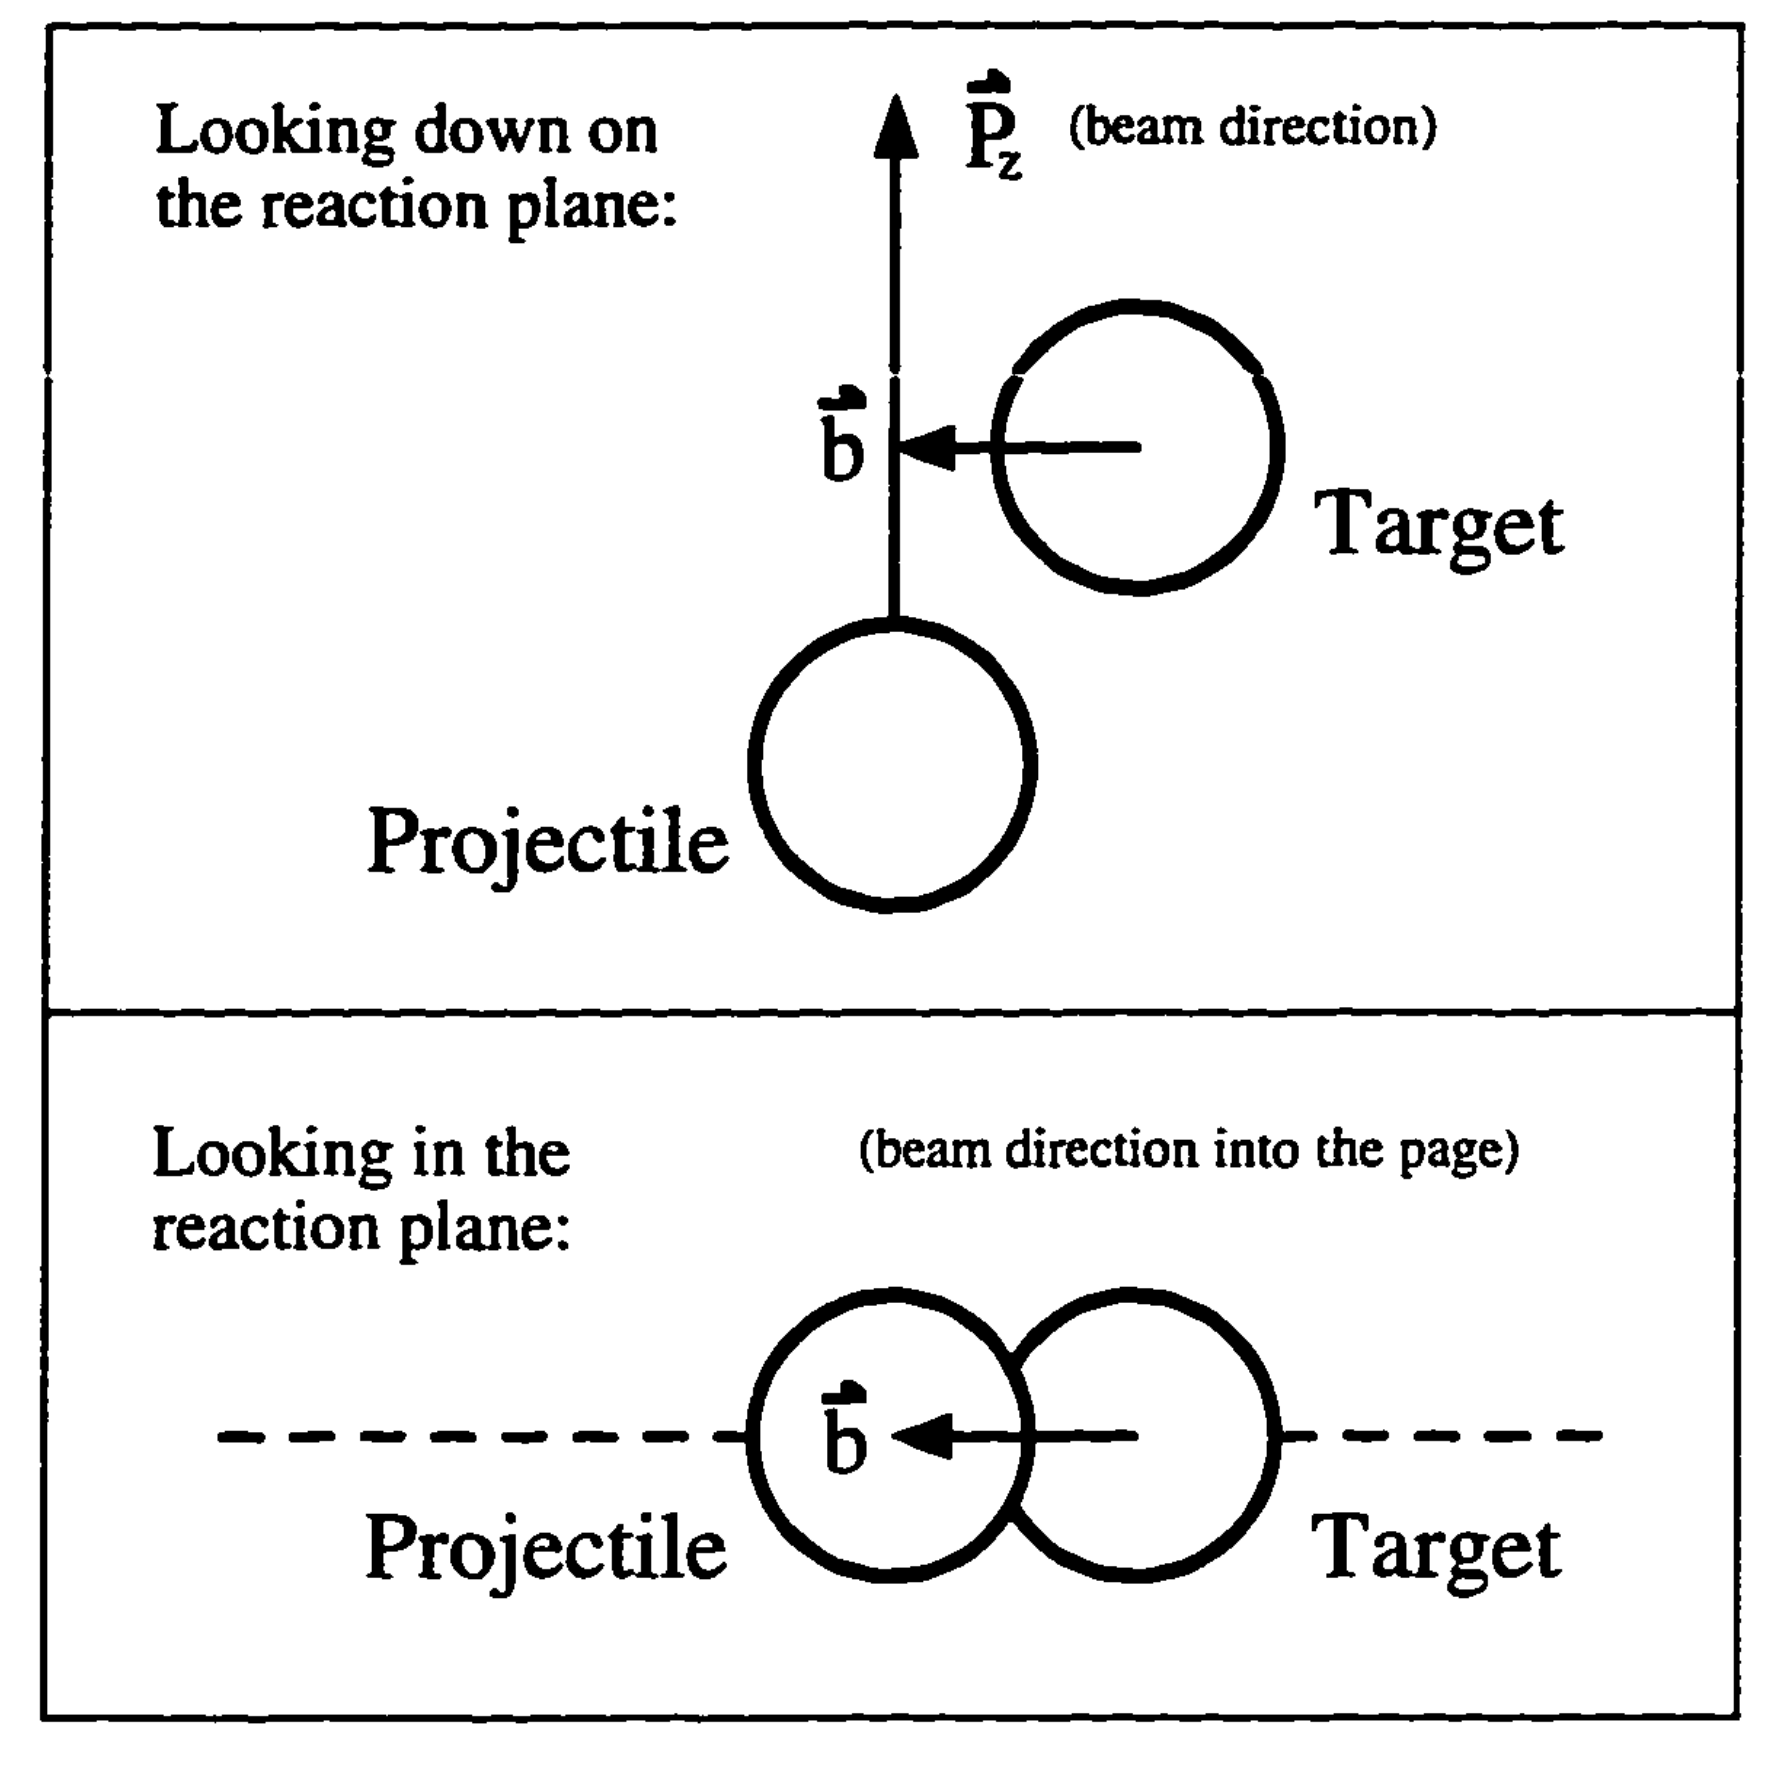
\includegraphics[width=\textwidth]{dad-thesis-figure}               
  One of the figures I helped my dad draw on a computer for his thesis, ``Collective flow in intermediate energy heavy-ion collisions,'' in 1996. Perhaps one day, I too will understand what it means.
\end{marginfigure}

\newthought{To my mother and father}, Dr. Robert and Myung-Hee Pak. My father, who was the first PhD in his own family, whom I remember happily marching down the aisles of the Breslin Center to the honks of Pomp and Circumstance for his doctorate in nuclear physics. Dad, you've been the role model for my life. Ever since I helped draw two figures for your thesis on the Macintosh you got me as a kid, proudly feeling like I had just put the torch on the Statue of Liberty, I've been wondering what it would be like to write one of my own. Well, have I got some bedtime reading material for you! And my mother, who kept me alive and kicking from a single cell all the way to whatever I am today, which if you think about it, is more remarkable than anything you will read in this dissertation. This never could have been written had it not been for my mother's ferocious dedication toward making a better life for me. Thanks, ma!

\newthought{To my thesis advisor}, Dr. Andrew Kasarskis, for taking me under his wing for the past four years. I am supremely lucky to have met somebody with the rare blend of patience, humor, genuine scientific curiosity, and mentorship skills that Andrew has and shares with others so freely. Andrew has taught me more than just science—he has taught me about leadership, entrepreneurship, integrity, life, and occassionally, wildlife. I look forward to pondering his lessons for the rest of my career. And to my fellow Kasarskis brother from the halls of Regis, the inimitable Dr. Joseph R. Scarpa, who blazed a trail for us both and kept me company as we jockeyed desks in Greenland. I am fortunate to be returning to medical school at his side.

\newthought{To the boys of 7G}, who are back in town, spread the word around. Kevin ``Carpet'' Hoffman, Michael ``The Stuffer'' Daniel, Zachary ``BJ'' Lorsch, Eddie ``Other Ted'' Contijoch, and Ranjan ``Gammie'' Upadhyay were my roommates as we began this strange and imprudent quest toward a dual degree. Then there's Andrew T. McKenzie, a late but profitable addition to the gang, who singlehandedly doubled our weirdness quotient and may just achieve his goal of a completely rational life strategy within the decade. And my entire entering class of 2012, who shall be rightfully remembered as ``the Titans.'' We have been through much together: retreats, pyramids, marathons, camping trips, uninhibited human flight, weddings, even a Tough Mudder—many of which could be considered a microcosm of certain aspects of the MSTP experience, but all of which I will always remember. You all kept me variously motivated, alive, and inspired throughout this ignoble quest, and I'll enjoy seeing you all crush it at science, medicine, and life.

\newthought{To the entire Sinai MSTP}, starting with the director from when I entered, Dr. Yasmin Hurd, and the many other leaders that have guided me since: Dr. Margaret Baron, Dr. Talia Swartz, Dr. Benjamin Chen, and Dr. Scott Friedman, to name a few. To the many other students in the program that gave me guidance and support, not least of all Dr. Benjamin Laitman, who was one of the first Sinai students I met, who steadfastly supported me through the challenges of leading Student Council, and whom I am honored to call my friend.

\newthought{To my colleagues in science}, who are also listed in acknowledgements within each chapter, but whom I must thank here not only for their collaborative efforts but also their friendship, mentorship, and personal support. From the Icahn Institute and Department for Genomics and Multiscale Biology: El-Ad David Amir, Oliver Attie, Ali Bashir, Harm van Bakel, Kieran Chacko, Brianne Ciferri, Gintaras Deikus, Gang Fang, Zeynep Gumus, Seunghee Kim-Schulze, Martha Lewis, David Nathanson, Leah C. Newman, Tim O'Donnell, Adeeb Rahman, Eric Schadt, Erick Scott, Robert Sebra, Mayte Suarez-Fariñas, Mitchell Sullivan, Maria Suprun, and Elizabeth Webster. From the Departments of Medicine and Pathology of the Mount Sinai Hospital: Judith Aberg, Camille Hamula, Jonathan Hand, Shirish Huprikar, Gopi Patel, Timothy Sullivan, and Fran Wallach. From the Department of Microbiology of the Icahn School of Medicine at Mount Sinai: Ana Fernandez-Sesma, Rebecca Hamlin, and Irene Ramos-Lopez, aka the Divas of Virology, who were so amazing to work with. To my colleagues from other institutions in the Dengue Human Immune Profiling Consortium, including Eva Harris and Daniela Michlmayr from UC Berkeley and Steven Wolinsky and Eun-Young Kim from Northwestern. There are likely many more scientists that quietly contributed their technical insight and effort to some aspect of the protocols, techniques, and datasets that eventually became a part of this dissertation, and for all of these unsung heroes whom I may never even meet, I want to express my sincere gratitude. 

\newthought{There are many other unsung heroes} in and around Mount Sinai whose support has been invaluable. Firstly, Courtney Manning, Gayle Schneiderman, and Rhaisili Rosario, who all did gangbusters work in keeping the MSTP running. Dr. Rainier P. Soriano, Dr. Yasmin Meah, Dr. David C. Thomas, Paul Lawrence, and Dr. David Muller gave me crucial guidance at certain points in the journey. I was lucky to have advice from Geoffrey Smith and Dan Seltzer on starting my business, The East Harlem Software Company, Inc. I have to thank the staff of Aron Hall, for maintaining such a nice home for all of us students. The guys at El Aguila on 103rd and Lex, whose tortas Cubanas fueled the improbable appearance of many words on these pages (which I recently learned is not an actual food in Cuba, but such is America). No acknowledgements could be complete without saluting Andy Efros, literally the nicest guy at Mount Sinai.

\newthought{I especially want to thank} Dr. Deena Altman for her dedicated leadership and evangelism of the Pathogen Surveillance Program, whose clinical insight and contributions made much of this dissertation possible before I even began, and who supported me from the first day I joined the group. As I go back into the hospital for clerkships and wonder what kind of doctor I want to be, I will be thinking often of Deena.

\newthought{To the members of my thesis advisory committee}: Dr. Adolfo García-Sastre, Dr. Jun Zhu, Dr. Joel Dudley, Dr. Jonathan Karr, and the chair Dr. James Iatridis, for providing focused guidance in developing this dissertation and meticulously supporting my development as a scientist. Special thanks to Dr. Bo Shopsin from the NYU School of Medicine, who graciously agreed to be an outside reviewer. To my undergraduate mentor, Dr. Frederick ``Fritz'' Roth, and members of his laboratory, who supported me throughout and after college, and first inspired me to pursue a doctorate in bioinformatics.

\newthought{Finally, I'd like to thank} Dr. Sonia Yen Jarrett, the only lady brave enough to put up with my shenanigans, who has kept me motivated throughout challenges I once thought impossible, and who always makes me laugh.

%%%%%%%%%%%%%%%%%%%%%%%%%%%%%%%%%%%%%%%%%%%%%%%%%%%%%%%%%%%%%%%%%%%%%%
% -*-latex-*-
  % -*- Mode:TeX -*-
%% This file simply contains the commands that actually generate the table of
%% contents and lists of figures and tables.  You can omit any or all of
%% these files by simply taking out the appropriate command.  For more
%% information on these files, see appendix C.3.3 of the LaTeX manual. 

\tableofcontents
%\newpage
\listoffigures
%\newpage
\listoftables

\cleardoublepage



%%
% We can set the line spacing for the main matter of the document using the toggles below.
% Note that after we do this, we then have to fix spacing between \marginpar's.
\mainmatter
%\doublespacing
\onehalfspacing
\setlength\marginparpush{12pt}
%% A chapter for my PhD dissertation
%% First author: Theodore Pak
%%
%% Must be included from main.tex.

\chapter{Introducing next-generation sequencing and multiscale data analysis into clinical infectious diseases}
\label{chap:intro}

\begin{quote}
\emph{Recent reviews have suggested that routine next-generation sequencing (NGS) on clinical specimens will improve the capabilities of clinical microbiology laboratories. However, the real opportunity to impact our understanding and management of infectious diseases lies in integrating NGS with clinical data from electronic medical records (EMRs), immune profiling data, and other rich datasets to create multiscale predictive models. This chapter introduces a range of new “omics” and patient data sources relevant to infectious diseases and proposes three potentially disruptive applications for these data in the clinical workflow. The combined threats of healthcare-associated infections and multidrug resistant organisms may be addressed by multiscale analysis of NGS and EMR data that is ideally updated and refined over time within each healthcare organization. Such data and analysis should form the cornerstone of future learning health systems for infectious disease.}
\end{quote}

\newthought{Next-generation sequencing} and “big data” analysis techniques are poised to transform our understanding of diseases that have a complex inherited component, such as cancer, diabetes, and heart failure. Perhaps even more significant, however, is the impact these technologies will have on the management of \emph{infectious diseases}, which have discrete, identifiable causes that can be isolated, cultured, and tested against drugs in vitro as part of a standard clinical workflow. Despite steady technological improvements in each step, this workflow’s principles have not changed for a century.\autocite{Didelot2012,Koser2012}

Our capacity to acquire “omics” data about infections is increasing exponentially. Nanoscale parallelization of DNA sequencing has precipitously dropped the cost per base-pair of finished genomes while increasing throughput, and the cost of sequencing and assembling a bacterial genome trends below \$100.\autocite{Didelot2012} PacBio RS sequencing has increased median read lengths over 10kbp, facilitating rapid, automated finishing of genomes for outbreak pathogens.\autocite{Chin2011,Rasko2011} Beyond sequencing pathogen genomes, recent studies have used other “omics” experimental techniques such as Luminex cytokine assays, RNA-seq, and mass cytometry to characterize immune responses to infection or vaccination with remarkable precision.\autocite{Mejias2014,Querec2009}

Many public databases curate and disseminate “omics” data relevant to infectious disease (Table \ref{tab:id_bioinf_dbs}), 
\begin{table*}[ht]
  \centering
  \small
  \begin{tabular}{p{3.5cm} l l l}
    \toprule
    \textbf{Database focus} & \multicolumn{1}{c}{For general research} & \multicolumn{2}{c}{For infectious disease}\\
    \cline{3-4}
    & & \multicolumn{1}{c}{Multi-pathogen} & \multicolumn{1}{c}{Pathogen-specific} \\
    \midrule
    Genomes &
    \begin{minipage}[t]{3.5cm}
      \raggedright
      \begin{itemize}[noitemsep]
      \item NCBI Nucleotide (GenBank/RefSeq)
      \item ENA/EMBL
      \item DDBJ
      \end{itemize}
    \end{minipage} & 
    \begin{minipage}[t]{3.5cm}
      \raggedright
      \begin{itemize}[noitemsep]
      \item ViPR
      \item NMPDR
      \item PATRIC
      \item EuPathDB
      \end{itemize}
    \end{minipage} & 
    \begin{minipage}[t]{3.5cm}
      \raggedright
      \begin{itemize}[noitemsep]
      \item Influenza Research Database (IRD)
      \item Tuberculosis Database (TBDB)
      \item LANL: Databases for HIV, HCV, and HFV 
      \end{itemize}
    \end{minipage}
    \\
    Gene products and functionality &
    \begin{minipage}[t]{3.5cm}
      \raggedright
      \begin{itemize}[noitemsep]
      \item UniProt
      \item KEGG
      \end{itemize}
    \end{minipage} &
    \begin{minipage}[t]{3.5cm}
      \raggedright
      \begin{itemize}[noitemsep]
      \item Pathogen-Host Interaction Database 
      \item Antibiotic Resistance Genes Database
      \item Comprehensive Antibiotic Resistance Database
      \end{itemize}
      \smallskip
    \end{minipage} &
    \\
    Expression and immune profiles &
    \begin{minipage}[t]{3.5cm}
      \raggedright
      \begin{itemize}[noitemsep]
      \item GEO
      \item ArrayExpress
      \end{itemize}
    \end{minipage} &
    \begin{minipage}[t]{3.5cm}
      \raggedright
      \begin{itemize}[noitemsep]
      \item ImmPort
      \end{itemize}
    \end{minipage} &
    \\
    \bottomrule
  \end{tabular}
  \caption[Bioinformatics databases for infectious diseases][12pt]{Examples of public bioinformatics databases that may be leveraged for multiscale analysis of infectious disease (this list is not exhaustive).}
  \label{tab:id_bioinf_dbs}
\end{table*}
but most lack significant clinical metadata. Increasing adoption of electronic medical records (EMRs) can potentially mitigate this problem because they typically include data on demographics, medications, lab results, and more. Figure \ref{fig:emr_sample_viz} presents a visualization of some of these datatypes as recorded by Mount Sinai Hospital’s EMR for two patients diagnosed with \textit{C. difficile} colitis.
\begin{figure}[htb]
  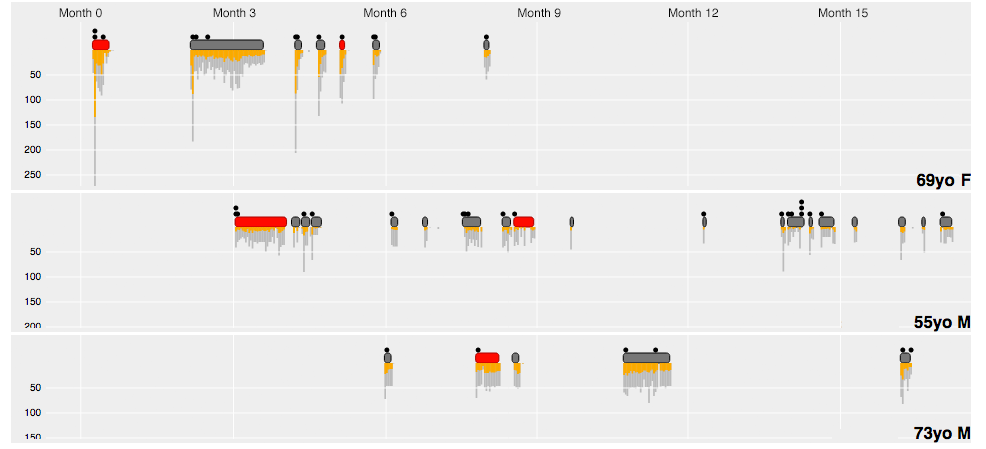
\includegraphics[width=\textwidth]{chap1/pt-timelines-deidentified}               
  \caption[Visualization of EMR data]{\textbf{Visualization of EMR data.} Timelines for two patients generated from EMR data in the Mount Sinai Data Warehouse (original analysis). Patient visits to Mount Sinai are represented as horizontal bars across the top of the timeline, and visits associated with a \textit{C. difficile} infection are highlighted in red.  The number of lab tests ordered per day is represented on the vertical axis, with abnormal results highlighted in orange.  Transfer events are marked by the black dots above the horizontal bars.}
  \label{fig:emr_sample_viz}
\end{figure}
With so many different stakeholders entering EMR data, however, automatically extracting certain facts (e.g., “this patient had the flu last Tuesday”) can be difficult. Nevertheless, high-accuracy methods for extracting infectious phenotypes such as influenza-like illness \sidecite[-1.2cm]{Silva2013}, unclear HIV status,\autocite{Felsen2014} and community-acquired pneumonia\autocite{DeLisle2013} have been demonstrated, and consortia such as eMERGE are standardizing comparison, validation, and deposition of these algorithms into a central repository.\autocite{Pathak2013a}

The marriage of real-time digital clinical information with “omics” technology creates the opportunity to increase the precision of clinical decision-making and challenges us to quickly design and execute bioinformatics analyses. Predictive modeling of infectious disease that incorporates EMR data is still rare, although one recent study generated a social network for hospital acquired infection from EMR data using recorded contacts between patients and caretakers.\autocite{Cusumano-Towner2013} Another found that statistical analysis of EMR data produces risk factors for C. difficile infection that outperform models based only on medically recognized risks.\autocite{Wiens2014} Likely because of the difficulty of integrating data across so many levels, no published studies have yet bridged predictive modeling on EMR data with pathogen genome sequences or other “omics” data from individual patients. Yet, for infectious disease, this is exactly what will fulfill the vision of a rapid-learning health system \autocite{Care2014,Kohane2012} that converts the informational byproducts of healthcare recorded by practitioners into evidence for future decision-making. While EMR data holds details of the clinical process and outcomes, “omics” data ties it back to pathophysiology and the precise strain and host-pathogen interactions present in each patient. Together, they can fuel a “learning engine” that integrates heterogeneous data into new clinical insights, interventions, and therapies. We will discuss how to leverage current bioinformatics software to build such an engine, and how this engine will be able to attack currently insurmountable problems in the field.

\section{The genomic clinical microbiology laboratory}

\newthought{Previous reviews}\autocite{Didelot2012,Koser2012} have proposed that cheap sequencing technology will transform clinical microbiology, while acknowledging technical and informational barriers to adoption. Whole genome sequencing (WGS) via NGS provides ultimate resolution for epidemiological studies of transmission and relatedness, and may soon be cost-effective for routine use.\autocite{Didelot2012,Koser2012} For pathogen identification, however, NGS is unlikely to usurp robotic culturing systems (e.g., Vitek and BD Phoenix) or newer mass spectrometry systems by cost and sensitivity comparisons alone, although it can lower turnaround time for difficult-to-culture organisms and identify novel or rarely-seen pathogens.\autocite{Koser2012,Naccache2015} Since susceptibility or resistance of an organism to drugs is in principle fully encoded in its genetic material \autocite{Didelot2012,Gordon2014}, NGS can also lower turnaround times for drug susceptibility testing of slow-growing organisms, such as M. tuberculosis \autocite{Boehme2010} and HIV-1.\autocite{Ram2015} This strategy should only expand as fuller catalogs of genomic variants that cause drug resistance are compiled for other pathogenic organisms.

\subsection{Leveraging existing bioinformatics tools}

An oft-mentioned hurdle\autocite{Didelot2012,Koser2012} for widespread use of NGS in clinical microbiology is the lack of readily accessible software for converting these data into species identifications, phylogenies, and drug susceptibilities. However, many mature open source bioinformatics solutions for individual components of these problems exist, and connecting these components into a pipeline is therefore a tractable software engineering exercise. Examples for most subtasks are listed in Table \ref{tab:id_bioinf_tools}. As NGS use by clinical microbiology laboratories becomes more commonplace, we might anticipate full-fledged genomic clinical microbiology software packages to become widely available.

\newthought{This expectation} has three foreseeable shortcomings. The first is that current tools are tied to centrally curated repositories of evidence. Although proponents of genomic clinical microbiology often envision encyclopedic databases hosted by international consortia,\autocite{Didelot2012,Koser2012} human curation is expensive and inefficient at scale, and many infectious diseases are locale-specific phenomena. Models based on pooled data may fail to reflect variation between healthcare delivery regions;\autocite{Reis2003,Wiens2014} for instance, a recent fitness model of H3N2 influenza based on international genomic surveillance data creates predictions only at the resolution of clades spanning multiple continents.\autocite{Luksza2014} Since implementation of NGS in a healthcare institution’s microbiology laboratory produces copious sequencing data not easily shared through public databases, institutions should prepare to manage repositories of local evidence and predictive models that work specifically for them. Over time, as data exchange interfaces are developed, institutions could form consortia to generalize analyses, which is a strategy that has successfully increased the power of human genome-wide association studies.\sidecite[-3em]{Gottesman2013,Kohane2012}

\begin{table}[ht]
  \centering
  \small
  \begin{tabular}{l l}
    \toprule
    \textbf{Problem domain} & \textbf{Software or database}\\
    \midrule
    Strain typing &
    \begin{minipage}[t]{5cm}
      \raggedright
      \begin{itemize}[noitemsep]
      \item Multi-Locus Sequence Typing (MLST) database
      \end{itemize}
      \smallskip
    \end{minipage}
    \\
    \textit{De novo} assembly from long reads &
    \begin{minipage}[t]{5cm}
      \raggedright
      \begin{itemize}[noitemsep]
      \item Celera
      \item Hierarchical Genome Assembly Process
      \end{itemize}
    \end{minipage}
    \\
    Species identification &
    \\
    \-\tabindent From clonal sample &
    \begin{minipage}[t]{5cm}
      \raggedright
      \begin{itemize}[noitemsep]
      \item NCBI BLAST
      \item GenBank
      \item Other databases in Table \ref{tab:id_bioinf_dbs}
      \end{itemize}
    \end{minipage}
    \\
    \-\tabindent From non-clonal sample &
    \\
    \-\tabindent\tabindent  Meta-assembly &
    \begin{minipage}[t]{5cm}
      \raggedright
      \begin{itemize}[noitemsep]
      \item AMOS
      \item MIRA
      \item MetaVelvet
      \end{itemize}
      \smallskip
    \end{minipage}
    \\
    \-\tabindent\tabindent Clustering and species annotation &
    \begin{minipage}[t]{5cm}
      \raggedright
      \begin{itemize}[noitemsep]
      \item MEGAN
      \item MG-RAST
      \end{itemize}
      \smallskip
    \end{minipage}
    \\
    Maximum likelihood phylogeny trees &
    \begin{minipage}[t]{5cm}
      \raggedright
      \begin{itemize}[noitemsep]
      \item BEAST
      \item RAxML
      \item ClonalFrame
      \item ClonalOrigin
      \end{itemize}
      \smallskip
    \end{minipage}
    \\
    Whole genome alignment &
    \\
    \-\tabindent For SNP calling &
    \begin{minipage}[t]{5cm}
      \raggedright
      \begin{itemize}[noitemsep]
      \item Mummer
      \item Mugsy
      \item Harvest
      \end{itemize}
      \smallskip
    \end{minipage}
    \\
    \-\tabindent For structural variant calling &
    \begin{minipage}[t]{5cm}
      \raggedright
      \begin{itemize}[noitemsep]
      \item Mauve
      \end{itemize}
      \smallskip
    \end{minipage}
    \\
    Gene annotation &
    \\
    \-\tabindent Bacterial &
    \begin{minipage}[t]{5cm}
      \raggedright
      \begin{itemize}[noitemsep]
      \item Glimmer
      \item RAST
      \item prokka
      \end{itemize}
      \smallskip
    \end{minipage}
    \\
    \-\tabindent Drug resistance in bacteria &
    \begin{minipage}[t]{5cm}
      \raggedright
      \begin{itemize}[noitemsep]
      \item Resfinder
      \item ARG-ANNOT
      \item Mykrobe predictor
      \end{itemize}
      \smallskip
    \end{minipage}
    \\
    \-\tabindent Other &
    \begin{minipage}[t]{5cm}
      \raggedright
      \begin{itemize}[noitemsep]
      \item Influenza Virus Sequence Annotation Tool
      \end{itemize}
      \smallskip
    \end{minipage}
    \\
    \bottomrule
  \end{tabular}
  \caption[Bioinformatics tools for infectious diseases]{Selected published bioinformatics software packages or databases that address specific steps of clinical microbiology tasks using NGS data (this list is not exhaustive). Well-established tools are available for many specific subtasks.}
  \label{tab:id_bioinf_tools}
\end{table}

A second shortcoming is that current pathogen annotation tools primarily make predictions using the simplistic criterion of sequence similarity. Machine learning (ML) algorithms could eventually integrate a wider array of genotypic features extractable from pathogen genomes—variant calls, putative gene and motif annotations, and more—and train holistic models that predict phenotypes. A “top-down,” integrative model predicting limited phenotypes from genotype for Mycoplasma genitalium is available;\autocite{Karr2012} top-down predictions of virulence, however, add the substantial complexity of host interactions. Therefore, genome-wide ML models of virulence have mostly been “bottom-up,” blind to mechanistic knowledge, and oriented toward even smaller-genome pathogens with considerable genomic surveillance data. ML on viral sequence features has predicted more effective antiretroviral combinations for HIV,\autocite{Lengauer2006,Zazzi2012} genetic markers for host selectivity within families of viruses,\autocite{Raj2011a} and optimal strain selection for H3N2 influenza vaccines.\autocite{Luksza2014} In general, given the explosion in available data, significant untapped potential remains for ML-based models that predict virulence, transmissibility, and drug resistance from pathogen genotypes. 

The third shortcoming is that for many common pathogens, these models are still limited by the paucity of clinical metadata linked to sequenced pathogens. Pathogen phenotypes accessible directly from EMRs include prognostic variables, such as length of stay and disposition, and lab results, such as drug susceptibilities. Although lab information systems (LIS) typically do not forward non-clinical results (e.g., growth curves) to EMRs, data exported from the LIS can help define richer phenotypes. For some diseases, EMRs will contain lab results that directly reflect infection severity, e.g., viral load for HCV and HIV patients,\autocite{Norton2014} while other diseases will require more complex criteria.\autocite{DeLisle2013,Klompas2008,Silva2013} Natural language processing of physician notes will facilitate the extraction of complex, high-accuracy clinical phenotypes from the EMR.\autocite{Liao2015,Silva2013} Routine NGS of specimens and EMR data on drugs prescribed and administered will enable ad-hoc studies crossing pathogen genotypes against interventions and outcomes. Richer characterization of particular host-pathogen encounters may be provided by immune and molecular profiling of selected patients, as well as animal experiments that establish individual pathogen genetic associations and molecular mechanisms. Biomarkers derived from such data\autocite{Mejias2014,Querec2009} could enhance predictive models built on a zealous integration of NGS and EMR data.

\newthought{The growth of EMR} phenotype information associated with pathogen genomes will spur a new generation of pathogenicity and risk models based on genomic data. Ideally, these models can drive a “learning engine” that integrates heterogeneous input data from an encounter with an infected patient and predict outcomes for possible interventions. Predictions can be delivered to physicians via clinical decision support systems that complement EMR functions by suggesting relevant actions within a patient’s electronic chart. The closing of the EMR–NGS–EMR loop (Figure \ref{fig:emr_ngs_loop}) should be the ultimate goal of bioinformatics pipelines for genomic clinical microbiology, because this would maximize the utility of data created for clinical encounters, continuously turning yesterday’s observations and outcomes into evidence for tomorrow’s predictions.\sidecite[-2em]{Care2014,Kohane2012}

\begin{figure}[htb]
  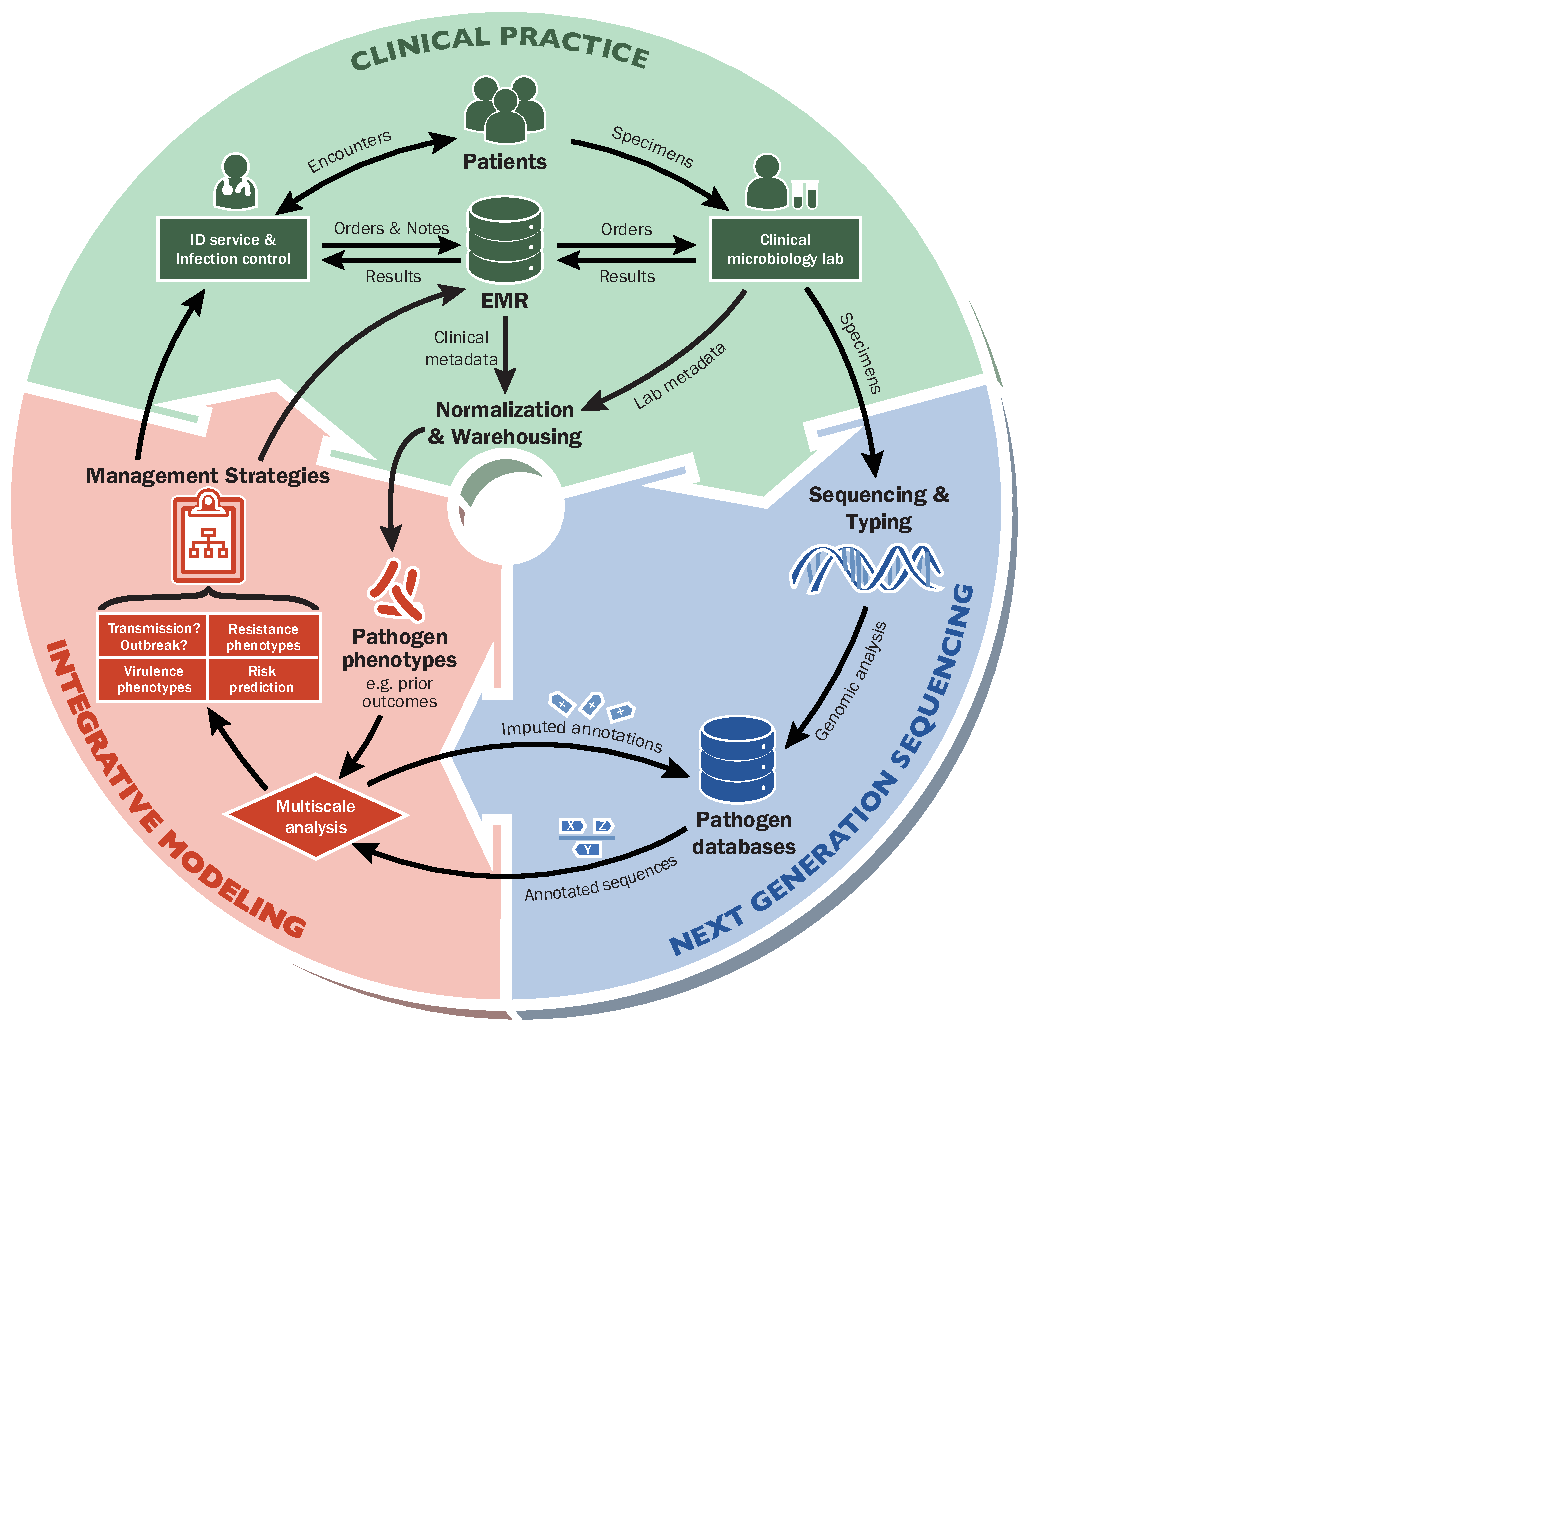
\includegraphics[width=\textwidth]{chap1/emr-ngs_loop_circular}               
  \caption[A learning health system for infectious diseases]{\textbf{A learning health system for infectious diseases.} Next generation sequencing (NGS) technologies now permit routine genomic analysis of clinical microbiology specimens. When integrated with pathogen phenotypes derived from clinical metadata in electronic medical records (EMRs) and laboratory metadata, we can generate predictive models for pathogen transmission, outbreaks, drug resistance, virulence, and risk factors for infection or critical outcomes that are specific to the health system and its patient population. If management strategies are formulated from these predictions and sent to infectious disease (ID) physicians and hospital infection control, a continuous loop of data analysis, application, and model refinement is created.}
  \label{fig:emr_ngs_loop}
\end{figure}

This sounds ambitious, but we can look to analogous software designed as subcomponents of learning healthcare systems to anticipate likely costs and avenues for development. The i2b2 platform\autocite{Kohane2012} and its counterpart SCILHS\autocite{Mandl2014} are vendor-agnostic solutions for extracting and unifying data across EMRs for reuse in cohort design and robust meta-analysis. The eMERGE consortium stimulated the creation of SHARPn for normalization and natural language processing of EMR data\autocite{Rea2012} and CLIPMERGE for automated pharmacogenomics alerts.\autocite{Gottesman2013} For these examples, working software was created after 1-5 years of development with \$100k-\$10M of annual public grant funding.\autocite{Gottesman2013,Kohane2012,Mandl2014,Rea2012} If the aforementioned open-source software is leveraged, an equal scale of public funding and collaboration among academic medical centers could make similar strides toward the proposal in Figure \ref{fig:emr_ngs_loop}. A modular framework allowed i2b2 to expand in scope organically after initial release,\autocite{Kohane2012,Mandl2014} suggesting that successful strategies should first aim for simple but clinically useful tasks such as identifying species and transmissions while anticipating the addition of more complex analyses via plugins and community contributions. In short, a reasonable investment in scrupulous software engineering could produce the seeds of a learning health system for infectious disease within the decade.

\section{Beyond genomic data}

\newthought{While NGS rapidly} moves toward routine use by clinical microbiology laboratories where it can be integrated with EMR data, other advances in data collection on infectious diseases create significant opportunities for predictive modeling that may eventually impact clinical practice. We now review these additional sources of data.

\subsection{Immune profiling}

Host response to infection is not merely the result of single gene modulations or amplification of specific cell types, but rather consists of complex interacting networks of RNA transcription, protein signaling and metabolism that impact cellular, tissue, and whole organism behaviors. The nature of the modulations that are specific to the host’s particular system relative to the state of the system at the time of infection ultimately determines risk and severity of disease. Recent studies have used “omics” scale experimental techniques to provide groundbreaking insight into immune responses, ranging from classification of acute respiratory infections in children\autocite{Mejias2014} and predicting immunogenicity of a vaccine\autocite{Querec2009,Furman2013} to characterizing effects of aging that gradually decrease vaccine efficacy.\autocite{Poland2014}

In each of these studies, researchers took an unbiased, hypothesis-free approach to their design and observed as many properties of the immune system as was experimentally feasible before, during, and after a perturbation, such as vaccine administration. Such properties include cytokine levels as measured by Luminex assays, global changes in gene expression within various leukocyte populations as measured by RNA-seq or microarrays, and changes in cell populations with various surface markers as observed by flow and mass cytometry. With sufficient sample size, patterns of biomarkers can be linked to various clinical outcomes, e.g., the host becoming immunogenic to an antigen. These biomarkers can then be investigated further for their functional role or used in new assays for point-of-care diagnosis. For common presenting conditions, like acute febrile illness, where current diagnostic methods poorly distinguish between bacterial and viral disease, this capability would allow prompt selection of the most appropriate therapy.\autocite{Mejias2014} For diseases like dengue that do not have accurate markers of immunization, these markers will be essential for development of a successful vaccine.\autocite{Mahalingam2013}

\subsection{The internet}

\begin{figure}[htb]
  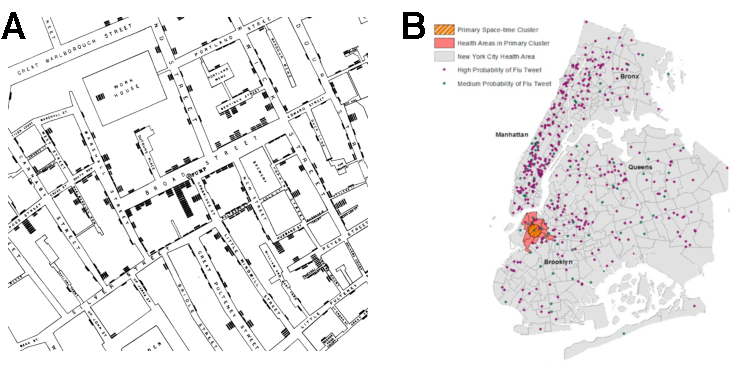
\includegraphics[width=\textwidth]{chap1/snow_and_new_combined}               
  \caption[Geospatial analysis, then and now]{\textbf{Geospatial analysis, then and now}. A, Excerpt from a map published by John Snow in 1855 depicting a cluster of cholera cases around a water pump on Broad Street in London, England. B, Retrospective analysis of geocoded tweets in New York City classified by the probability of representing actual influenza cases during the 2012-2013 flu season, from \textcite{Nagar2014}. The primary outbreak cluster was determined to be in Northern Brooklyn.}
  \label{fig:snow_and_new_combined}
\end{figure}

Patients can now be associated with a trove of digitized information that can be mined to better understand infectious disease. Frequent social contacts are often captured in address books, email inboxes, and social networks like Facebook. Patients discuss symptoms online, which have been captured from search engine queries\autocite{Ginsberg2009} or public Twitter streams to find probable cases of pertussis, whooping cough, and influenza,\autocite{Nagel2013} although these studies have known limitations.\autocite{Lazer2014} Often this data is attached to geospatial information, which can be used to construct spatiotemporal models of the disease that reveal clusters and the directionality  of spread within a city environment,\autocite{Nagar2014} providing in real time the same type of analysis that 19th century anesthesiologist John Snow meticulously compiled to identify a London water pump handle as the source of a cholera outbreak (see Figure \ref{fig:snow_and_new_combined}).\autocite{Buechner2004,Snow1855} Global human movement patterns are also captured in air travel network usage data, which has previously been combined with genomic surveillance data to predict transmission dynamics of H3N2 influenza.\autocite{Lemey2014} Unifying such diverse data in clinically relevant models with actionable outputs remains a significant challenge. On the other hand, the advent of cloud computing and open-source data science platforms like Apache Hadoop, used by Facebook and Walmart to model complex consumer behavior, suggests that algorithms for large, heterogeneous datasets will become increasingly accessible to healthcare providers and life sciences researchers.\autocite{Mohammed2014}

\section{Impact on clinical management}

\newthought{Three potential applications} of a new learning healthcare system for infectious diseases could address some of the most urgent global problems in infectious disease. One problem is rising antimicrobial resistance, which the World Health Organization names one of the three greatest threats to human health.\autocite{Policy2010} Care providers overusing antimicrobials and fomenting resistance in subclinical carriers are partly to blame, with recent studies estimating the fraction of misuse to be between quarter to half of all treatments.\autocite{McKellar2014} Multidrug resistance increases the morbidity and mortality of healthcare-acquired infections (HAIs), which have an incidence of 1.7 million cases per year in the US and an estimated annual cost of more than \$30 billion \autocite{Scott2009} that dwarfs the likely cost of any informatics-based preventative efforts. The sobering threat of extensively drug-resistant community-circulating organisms, some of which have therapeutic failure rates of 25-29\%,\autocite{Hirsch2010} alters the risk analysis for hospital procedures once considered routine and calls for comprehensive new strategies for management.

\subsection{Identifying high-risk patients for HAI}

Infection control for HAIs depends on identifying high-risk patients and applying isolation precautions or reducing known risk factors during their hospital course. For C. difficile infection (CDI), the most frequently reported nosocomial infection in the US, many questions about how infections are acquired and managing at-risk patients remain.\autocite{Leffler2015} The prevailing notion that infections are mostly transmitted person-to-person within hospitals \autocite{Cohen2010} conflicts with recent NGS evidence that sources of infection are more diverse,\autocite{Eyre2013} suggesting a greater role for asymptomatic colonized patients and environmental sources.

Each healthcare system represents a unique milieu of person-to-person contact networks, contaminated surfaces, microbiomes, and asymptomatic colonization that contributes to the risk of CDI. EMR and NGS data can prove or disprove transmission between patients and unlock the secrets of modifiable risk factors in this chaotic environment. ML algorithms predicting individual risk of CDI for a large hospital performed better (area under receiver operator curve, AUC=0.81) when operating on >10,000 unconstrained EMR variables rather than curated variables for known risk factors.\autocite{Wiens2014} Similar ML models based on EMR data between 2009-2014 for The Mount Sinai Hospital in New York City, encompassing 192,000 patients and 1,366 CDI diagnoses, show equal performance (AUC=0.80) and draw out associations not typically published for CDI. These may be unique to Mount Sinai’s environment and include respiratory failure (odds ratio OR=8.3, 95\% confidence interval 6.6-10.3), nutritional irregularity (OR=6.6, 4.7-8.6), and pancytopenia (OR=4.4, 3.1-5.5) (Timothy O’Donnell, personal communication).

A model-based decision support system would screen patients with higher CDI or asymptomatic colonization likelihood and allow earlier diagnosis and intervention. NGS-confirmed transmission events and interactions between people and equipment seen in the EMR and other data could extend this basic model to highlight common factors behind verified transmission and inform empirical, real-time modifications of infection control policy. Cross-sectional analysis by NGS-derived phenotypes and risk factors in the EMR would facilitate more precise clinical decision-making, for instance, whether shortening patient time in intensive care units or decreasing use of provocative antibiotics would be more preventative within the local milieu.  Short of a clinical trial that is probably infeasible to conduct, much less replicate across institutions, there is scant evidence for making these decisions at present, so a localized quantitative model can only help.

\subsection{Earlier detection of outbreaks inside and outside the hospital}

Current infection control software suites like VigiLanz Dynamic Monitoring Suite and TheraDoc Infection Control Assistant primarily issue outbreak alerts based on infection frequency thresholds. This could be rendered obsolete by routine NGS of clinical microbiology specimens, which determines with great precision whether a transmission event has occurred.\autocite{Didelot2012,Koser2012} A software system with access to EMR and other hospital data could automatically search elements common between verified transmission cases (caregivers, equipment, or rooms) and alert staff to inspect these elements before they produce enough transmissions to trigger a frequency threshold alert. Given enough historical data, NGS could also help hospitals differentiate community- from hospital-acquired infections and thereby refine metrics used to evaluate infection control policies.

An active effort to sample the environment inside and outside the hospital could further extend the reach of this surveillance. Within the hospital, “problem spots” identified by earlier investigations could be resampled regularly via NGS to re-evaluate the efficacy of infection control measures. The hospital also samples the pathogen ecosystem of the local population. Hospitals already report diagnoses of highly transmissible and dangerous infections to government authorities, and sharing NGS data for these cases would permit real-time assessment of where pathogens are coming from, how they are evolving, and where populations naïve to a pathogen are located. Current mapping and surveillance efforts \autocite{Brownstein2008} would be vastly enhanced by rich phylogenetic information, allowing outbreaks across disparate regions to be linked.\autocite{Chin2011,McAdam2012,Rasko2011} Fine-grained, real-time tracking of infectious disease spread would better inform doctors diagnosing and treating new patients, field agents tracking cases and contacts, and health policymakers seeking preventive population measures.

\subsection{Antimicrobial stewardship}

Decision support systems for empirical antibiotic therapy have been investigated for decades,\autocite{Leibovici1997} but with the prevalence of antimicrobial resistance skyrocketing, the urgency to implement systems that specifically encourage restraint with antibiotics has increased.\autocite{Wagner2014} Selective reporting is a common strategy that directs providers toward optimal therapies simply by omitting names of inappropriate drugs in susceptibility reports.\autocite{Doern2013} A more aggressive strategy pushes EMR alerts whenever physicians prescribe antibiotic treatment inconsistent with best practices.\autocite{Kullar2013}

These solutions ignore the power of the EMR to provide evidence that justifies or improves the antimicrobial stewardship interventions. For instance, although it is well accepted that antibiotic overuse increases the prevalence of resistance, current antimicrobial stewardship programs have demonstrated neither effects on patient outcomes nor even that decreased antibiotic treatment leads to decreased antibiotic resistance.\autocite{Wagner2014} By integrating NGS and EMR data, these hypotheses could be investigated in minute detail within large patient cohorts. NGS can reveal and enumerate the genetic mechanisms of resistance circulating through a health system. By tracing the recurrence of pathogens in the local community, an NGS-equipped health system can determine whether patients receiving antibiotics have generated and transmitted drug-resistant mutants. Specific drug regimens can be correlated with the development of particular resistance mutations. Conversely, given enough longitudinal data, the efforts of an antimicrobial stewardship program can be validated by observing decreased emergence of resistance mutations to drugs prescribed more conservatively.

\section{Conclusions}

\newthought{Routine access} to pathogen genomic data will transform our ability to manage infections, but only if we can integrate this information with clinical and other data to power predictive models for critical outcomes. Assuming that the hurdles of cost, accuracy, and turnaround time can be addressed, which is likely given current trends, NGS will soon become a standard clinical microbiology procedure. The unprecedented specificity of this data will in the near term allow reconstruction of transmission networks inside and outside of hospitals. In the far term, having rich clinical data linked to pathogen genotypes will permit predictions of prognosis, virulence, and drug susceptibility for active infections once NGS data is available. Incorporating these capabilities into a new clinical workflow that actively refines predictive models by adjusting to new data (Figure \ref{fig:emr_ngs_loop}) should improve case management, risk prediction for HAIs, detection of outbreaks, and antimicrobial stewardship. The missing link in this transformation, and the goal for bringing it to fruition, is software that leverages best-of-breed existing tools, incorporates all relevant heterogeneous datatypes, builds on electronic phenotyping algorithms to scrub low-accuracy EMR data, and validates against gold standard clinical case review.
Healthcare institutions and researchers should recognize that a potent combination of NGS and EMR data will transform infectious disease management. The threats posed by multidrug resistance and healthcare associated infections demand a revolution in management strategy. Predictive modeling grounded in rich, diverse molecular and clinical data will dramatically increase the precision of care and help hold these threats at bay.

\section*{Notes}

A shortened version of this chapter was published in \textit{Clinical Infectious Diseases}.\autocite{Pak2015}

\subsection{Acknowledgements}

We thank Deena Altman and Shirish Huprikar for critical suggestions on the manuscript.

\subsection{Financial support}

The authors were supported by the Icahn Institute for Genomics and Multiscale Biology at Mount Sinai.

\subsection{Potential conflicts of interest}
We certify no potential conflicts of interest.

%% This is an example first chapter.  You should put chapter/appendix that you
%% write into a separate file, and add a line \include{yourfilename} to
%% main.tex, where `yourfilename.tex' is the name of the chapter/appendix file.
%% You can process specific files by typing their names in at the 
%% \files=
%% prompt when you run the file main.tex through LaTeX.

\chapter{Whole-genome sequencing identifies emergence of a quinolone resistance mutation in a case of \emph{Stenotrophomonas maltophilia} bacteremia}
\label{chap:steno}

\begin{quote}
\emph{In this chapter we use next-generation sequencing to reveal the mechanism of emerging drug resistance in a case of hospital-acquired infection following the failure of routine antimicrobial therapy. Whole genome sequences for \emph{Stenotrophomonas maltophilia} serial isolates from a bacteremic patient before and after development of levofloxacin resistance were assembled \emph{de novo} and differed by one single-nucleotide variant in \emph{smeT}, a repressor for multidrug efflux operon \emph{smeDEF}. Along with sequenced isolates from five contemporaneous cases, they displayed considerable diversity compared against all previously published complete genomes. Whole genome sequencing and complete assembly can conclusively identify resistance mechanisms emerging in \emph{S. maltophilia} strains during clinical therapy.}
\end{quote}

\section{Introduction}

\emph{Stenotrophomonas maltophilia} is an aerobic, non-fermenting, and motile Gram-negative bacterium that is increasingly recognized as a cause of hospital-acquired infections with crude mortality rates of 14–69\% in cases of bacteremia.\autocite{Brooke2012} Treatment of \emph{S. maltophilia} infections is challenging due to the pathogen’s intrinsic resistance to many antibiotic classes via drug efflux pumps, beta-lactamase production, and decreased membrane permeability.\autocite{Brooke2012} Resistance phenotypes are known to change during the course of treatment, which complicates interpretation of automated drug susceptibility testing (DST) results.\autocite{Garrison1996} A mutant strain of \emph{S. maltophilia} with emerging resistance to tetracycline, chloramphenicol, and quinolones was previously characterized following in vitro tetracycline selection.\autocite{Alonso1997,Sanchez2002} However, little is known about the genetic and molecular mechanisms underlying acquired resistance in the clinical setting—particularly for quinolones, where in contrast to other Gram-negatives, the quinolone-resistance determining region (QRDR) of topoisomerase genes is often unaltered.\autocite{Valdezate2005} In this report, we describe the first reported use of whole genome sequencing (WGS) in serial clinical isolates to definitively identify an acquired quinolone resistance mutation in \emph{S. maltophilia}. WGS was performed for the initial and subsequent \emph{S. maltophilia} blood culture isolates from a patient where acquired quinolone resistance was observed (Patient 1) and five other patients (Patients 2-6) selected from a two-month period in 2013 at The Mount Sinai Hospital. 

\section{Case report}

Patient 1 was a 56 year-old man with a history of pancreatic cancer and a Whipple procedure eleven years earlier who presented to The Mount Sinai Hospital with variceal bleeding at the hepaticojejunostomy site. A transjugular intrahepatic portosystemic shunt was placed, which was complicated by thrombosis. In the following weeks, he had several episodes of polymicrobial bacteremia and was treated with multiple courses of antimicrobials, including a 10-day course of levofloxacin. Two months after levofloxacin exposure, he developed another episode of polymicrobial bacteremia. Blood cultures intermittently grew \emph{S. maltophilia}, \emph{E. faecium}, and \emph{Candida parapsilosis} despite appropriate antimicrobial therapy. Automated DST showed that the first \emph{S. maltophilia} isolate acquired was susceptible to levofloxacin (minimum inhibitory concentration [MIC] 0.5µg/mL) and trimethoprim/sulfamethoxazole (TMP-SMX; MIC ≤20 µg/mL). He was treated with 400 mg intravenous ciprofloxacin every 8 hours, but blood cultures nine days later again grew \emph{S. maltophilia}, now resistant to levofloxacin (MIC >32µg/mL) while still susceptible to TMP-SMX (MIC 1µg/mL). Ciprofloxacin therapy was stopped and intravenous TMP-SMX was given every 8 hours; subsequent cultures did not grow \emph{S. maltophilia}.

\section{Methods}

Standard culturing and susceptibility testing for levofloxacin and SXT were performed by automated microbroth dilution with Vitek2® (bioMérieux). Antimicrobial sensitivities were reported and interpreted according to the 2015 CLSI guidelines for \emph{S. maltophilia}.\autocite{ClinicalandLaboratoryStandardsInstitute2015} Isolates were then stocked and frozen at -80°C. Levofloxacin and SXT susceptibilities for all isolates in this study were later confirmed by Etest (bioMérieux) at 24 hours. To prepare for sequencing, isolates were grown from single colonies in tryptic soy broth, and DNA extraction was performed as previously described.\autocite{Altman2014}

\subsection{Genome sequencing}

Sequencing was performed to a depth of coverage of >150x per genome using the P4-C2 sequencing enzyme and chemistry at the manufacturer’s specifications on the PacBio RSII platform (Pacific Biosciences, Menlo Park, CA). For ISMMS2 and ISMMS2R, Sanger sequencing was additionally performed on six PCR-amplified regions encompassing the one single nucleotide variant (SNV) and five one-base indels that differentiated the two PacBio assemblies. Conventional PCR amplification was performed with Choice-Taq Blue (Denville Scientific) and included an initial denaturation step of 180s at 95°C, 30 cycles of denaturation, annealing, and extension at 95°C/30s, 60°C/30s, and 72°C/30s respectively, and a final extension step of 300s at 72°C. Primer sequences are as follows: for the SNV, \texttt{5’-CAAGGTGCTGACCGAAATGC-3’} forward and \texttt{5’-ACACGCCATCCTTCACGTAG-3’} reverse; and for the five indels, \texttt{5’-GCATGGAAGTACCACTGGGT-3’} forward + \texttt{5’-TTGGAGGGGTGGTAAAACGG-3’} reverse, \texttt{5’-TGGCCAACCCCTTCTATGTC-3’} forward + \texttt{5’-CCATGGCCACAGCAAAATGG-3’} reverse, \texttt{5’-CTGCCTTCGGTCACTTCGT-3’} forward + \texttt{5’-TGGAAGTCTCGCTGGAAGGT-3’} reverse, \texttt{5’-GCCCTCTACACCGTCTTTCC-3’} forward + \texttt{5’-GAACTACCGGACGGCTTTGA-3’} reverse, and \texttt{5’-AACTTCTTCGTGTCGGTCCC-3’} forward + \texttt{5’-AGAACTACCGGACGGCTTTG-3’} reverse. Sequences on both strands of the amplified products were determined at an external sequencing facility (Macrogen Inc., Rockville, MD) using the standard Sanger dideoxy-terminator method and the same primers.

\subsection{Sequence assembly and annotation}

Sequencing data was processed and assembled de novo using PacBio’s Hierarchical Genome Assembly Process\autocite{Chin2013} (HGAP, version 3) in the SMRTanalysis toolkit (version 2.3.0) using standard pre-assembly pipeline parameters. Custom scripts were used to circularize the draft assemblies and orient them similarly to reference assemblies K279a, R551-3, D457, and JV3 using the \emph{gyrB} locus as a landmark; these scripts are available at \url{https://github.com/powerpak/pathogendb-pipeline/releases/tag/steno\_v1.0} (\textsc{doi}:\href{http://dx.doi.org/10.5281/zenodo.17295}{10.5281/zenodo.17295}) within the files \texttt{scripts/circularizeContigs.pl} and \texttt{scripts/fasta-orient-to-landmark.pl}. To eliminate overhanging sequence at the end of contigs and to increase accuracy, raw reads were re-mapped to the circularized assemblies using Blasr and the final consensus was re-called using Quiver. Initial annotations were created using the RAST server\autocite{Overbeek2014} with specific annotation of sme genes derived from BLAST queries.
Depth of coverage reported in Table 1 was calculated by SMRTanalysis (version 2.3.0) during re-mapping of reads to the circularized draft assembly.

\subsection{Accession numbers}

Sequences and annotations for reference assemblies of clinical \emph{S. maltophilia} isolates K279a, R551-3, D457, and JV3 were obtained from GenBank/RefSeq at accession numbers \texttt{AM743169.1}, \texttt{NC\_011071.1}, \texttt{NC\_017671.1}, and \texttt{NC\_015947.1}, respectively. These represent the entirety of assemblies for \emph{S. maltophilia} found in NCBI Assembly with an Assembly Level of “Complete Genome” (\url{http://www.ncbi.nlm.nih.gov/assembly/organism/40324/all/}) at the time of the study.\footnote{By 2017, excepting the three assemblies submitted as a result of this study, only one more complete genome (\href{https://www.ncbi.nlm.nih.gov/assembly/GCF\_002025605.1/}{ASM202560v1}) is available.} K279a and D457 were isolated from human infections, while R551-3 and JV3 were isolated from plants. Previously published sequences for the quinolone-resistance determining region (QRDR) of the \emph{gyrA}, \emph{gyrB}, \emph{parC} and \emph{parE} genes in \emph{S. maltophilia}\autocite{Valdezate2002} were obtained from EMBL/European Nucleotide Archive.

Complete genome sequences for ISMMS2, ISMMS2R, and ISMMS3 were deposited in GenBank at accession numbers \texttt{CP011305}, \texttt{CP011306}, and \texttt{CP011010}, respectively. Deposited sequences for ISMMS2 and ISMMS2R incorporate the Sanger corrected regions described above. Sequences for ISMMS4, ISMMS5, ISMMS6, and ISMMS7 were deposited as Whole Genome Shotgun projects at DDBJ/EMBL/GenBank under the accessions \texttt{JZIU00000000}, \texttt{JZIV00000000}, \texttt{JZIW00000000}, and \texttt{JZTX00000000}, respectively, with the versions described in this chapter at \texttt{JZIU01000000}, \texttt{JZIV01000000}, \texttt{JZIW01000000}, and \texttt{JZTX01000000}, respectively.

\subsection{Comparative genomic analysis}

Pairwise comparison between strains was performed with the MUMmer 3.23 package,\autocite{Delcher2003} firstly using nucmer for pairwise genome alignment. The resulting nucmer alignments were filtered for quality and uniqueness via the \texttt{delta-filter} tool (using the \texttt{–1} flag to identify top alignments between the reference and query intervals). To estimate phylogenetic tree distances, high-quality SNP and indel calls were assigned via the \texttt{show-SNPs} tool using the \texttt{–C} flag to only report SNPs in regions with unambiguous mappings. For ISMMS2 and ISMMS2R, \texttt{show-SNPs} was also used without the \texttt{–C} flag to verify that no additional SNPs or indels were in ambiguously mapped regions.

Mugsy version 2.2 was used to perform multiple sequence alignment of the whole genome sequences in order to find local collinear blocks (LCBs) of conserved sequence.\autocite{Angiuoli2011} These aligned blocks were used to establish a core genome (of 3.01 Mbp) across all isolates, from which a phylogenetic tree was constructed using RAxML version 8.0.2,\autocite{Stamatakis2014} employing the GTRGAMMA substitution model and performing 20 runs. Whole genome alignments for visualization of recombination events was performed with Mauve 2.4.0,\autocite{Darling2004} using the \emph{progressiveMauve} algorithm\autocite{Darling2010} with a minimum seed weight of 21, seed families enabled, and all other parameters at defaults. Clustal Omega\autocite{Sievers2011} was used for multiple sequence alignment of putative amino acid sequences, which were then rendered with ESPript version 3.0.\autocite{Robert2014}

\subsection{Epigenetic motif analysis}

For each isolate, initial DNA modification motifs were first predicted by a de novo motif discovery pipeline in SMRTportal (\texttt{RS\_Modifications\_Motif\_Analysis.1}). The pipeline searches for kinetic variations in DNA polymerization events recorded during sequencing that correlate with modifications in the template, with different modifications creating distinct kinetic profiles.\autocite{Clark2012,Fang2012} At the coverage depths reported for this study, the probability (power) of detecting a modification event at a site at the 0.1 significance threshold, if it is truly modified, exceeds 99.99\%.\autocite{Fang2012} Raw predictions, which often have incorrectly- or over-called motifs, were further refined by a re-analysis of the raw data using a single molecule level characterization method.\autocite{Beaulaurier2015} Conceptually, this method was used to check the single molecule level methylation status of each putative motif and its neighboring (more or less specific) motifs and determine the real motif. 

\section{Results}

Two complete whole genome sequences were derived from Patient 1’s isolates before and after the change in levofloxacin MIC and compared to whole genome sequences of five control \emph{S. maltophilia} isolates (Patients 2-6). All sequences were \emph{de novo} assembled, i.e., without regard to reference assemblies. Table \ref{tab:steno_pts} summarizes the relative dates of collection, antimicrobial susceptibility results, and assembly statistics.

\newcommand{\PreserveBackslash}[1]{\let\temp=\\#1\let\\=\temp}
\newcolumntype{P}[1]{>{\PreserveBackslash\raggedright}p{#1}}

\begin{table*}[ht]
  \centering
  \small
  \begin{flushleft}
  \begin{tabular}{l P{1.5cm} P{1.5cm} l l l l P{2.5cm} P{1.5cm}}
    \toprule
    \multirow{2}{*}{Patient} & 
    \multirow{2}{1.5cm}{Time of collection (days)$^a$} &
    \multirow{2}{1.5cm}{Isolate name} &
    \multicolumn{2}{P{3cm}}{Levo susceptibility (MIC, mg/L)} &
    \multicolumn{2}{P{3cm}}{SXT susceptibility (MIC, mg/L)} &
    \multirow{2}{2.5cm}{Assembly quality} &
    \multirow{2}{1.5cm}{Depth of coverage}
    \\
    \cmidrule(r){4-5}\cmidrule(r){6-7}
    & & & Vitek2 & Etest & Vitek2 & Etest & &
    \\
    \midrule
    1  &  0   & ISMMS2  &  S (0.5)$^b$ &  S (1)     & S (<20)      & S (0.19) & 1 circular 4.51Mbp chromosome & 160x \\
    1  &  +10 & ISMMS2R &  R (>32)$^b$ &  R (16)    & S (1)        & S (0.38) & 1 circular 4.51Mbp chromosome & 403x \\
    2  &  -26 & ISMMS3  &  S (0.25)  &  S (0.38)  & U (80, <20)$^c$ & S (0.75) & 1 circular 4.80Mbp chromosome & 153x \\
    3  &  +14 & ISMMS4  &  R (>8)    &  R (>12)   & U (0.5, 80)$^c$ & S (0.75) & 3 contigs (4.73Mbp, 6.5kbp, 11.2kbp) & 303x \\
    4  &  -32 & ISMMS5  &  S (1)     &  S (1)     & S (<20)      & S (0.25) & 18 contigs & 270x\\
    5  &  0   & ISMMS6  &  S (<0.12) &  S (0.125) & S (<20)      & S (1.5)  & 10 contigs & 262x\\
    6  &  +2  & ISMMS7  &  S (1)     &  S (0.75)  & S (<20)      & S (1.5)  & 1 circular 4.69Mbp chromosome, 1 additional 17.7kbp contig & 318x\\
    \bottomrule
  \end{tabular}
  \end{flushleft}
  \caption[Sequenced clinical isolates and their antimicrobial susceptibilities]{Sequenced clinical isolates and their antimicrobial susceptibilities. Abbreviations: Levo, levofloxacin; SXT, trimethoprim/sulfamethoxazole; S, susceptible; R, resistant; U, undetermined; Mbp, million base pairs; kbp, thousand base pairs. $^a$Time of collection was defined in days relative to the date of collecting the initial \emph{S. maltophilia} isolate in the case patient. $^b$This is the change in levofloxacin susceptibility investigated in this study. $^c$Inconsistent results were obtained in replicate.}
  \label{tab:steno_pts}
\end{table*}

\subsection{Emergence of a point mutation conferring quinolone resistance}

Assembled genome sequences for Patient 1’s isolates before (ISMMS2) and after (ISMMS2R) observation of levofloxacin resistance were compared directly and were identical except for one single-nucleotide variant (SNV) and five one-base indels. Sanger sequencing confirmed the presence of the SNV, but identified the indels as homopolymer assembly errors. Coding domain sequence predictions for the surrounding locus (Figure \ref{fig:snp_location}A) revealed that the SNV was inside \emph{smeT}, a \emph{tetR}-like repressor upstream of the structural operon for the \emph{smeDEF} genes, which encode a multidrug efflux pump. The SNV is an A>T substitution at position 497 of \emph{smeT} causing a nonsynonymous Leu-166→Gln mutation.

\begin{figure*}[tbp]
  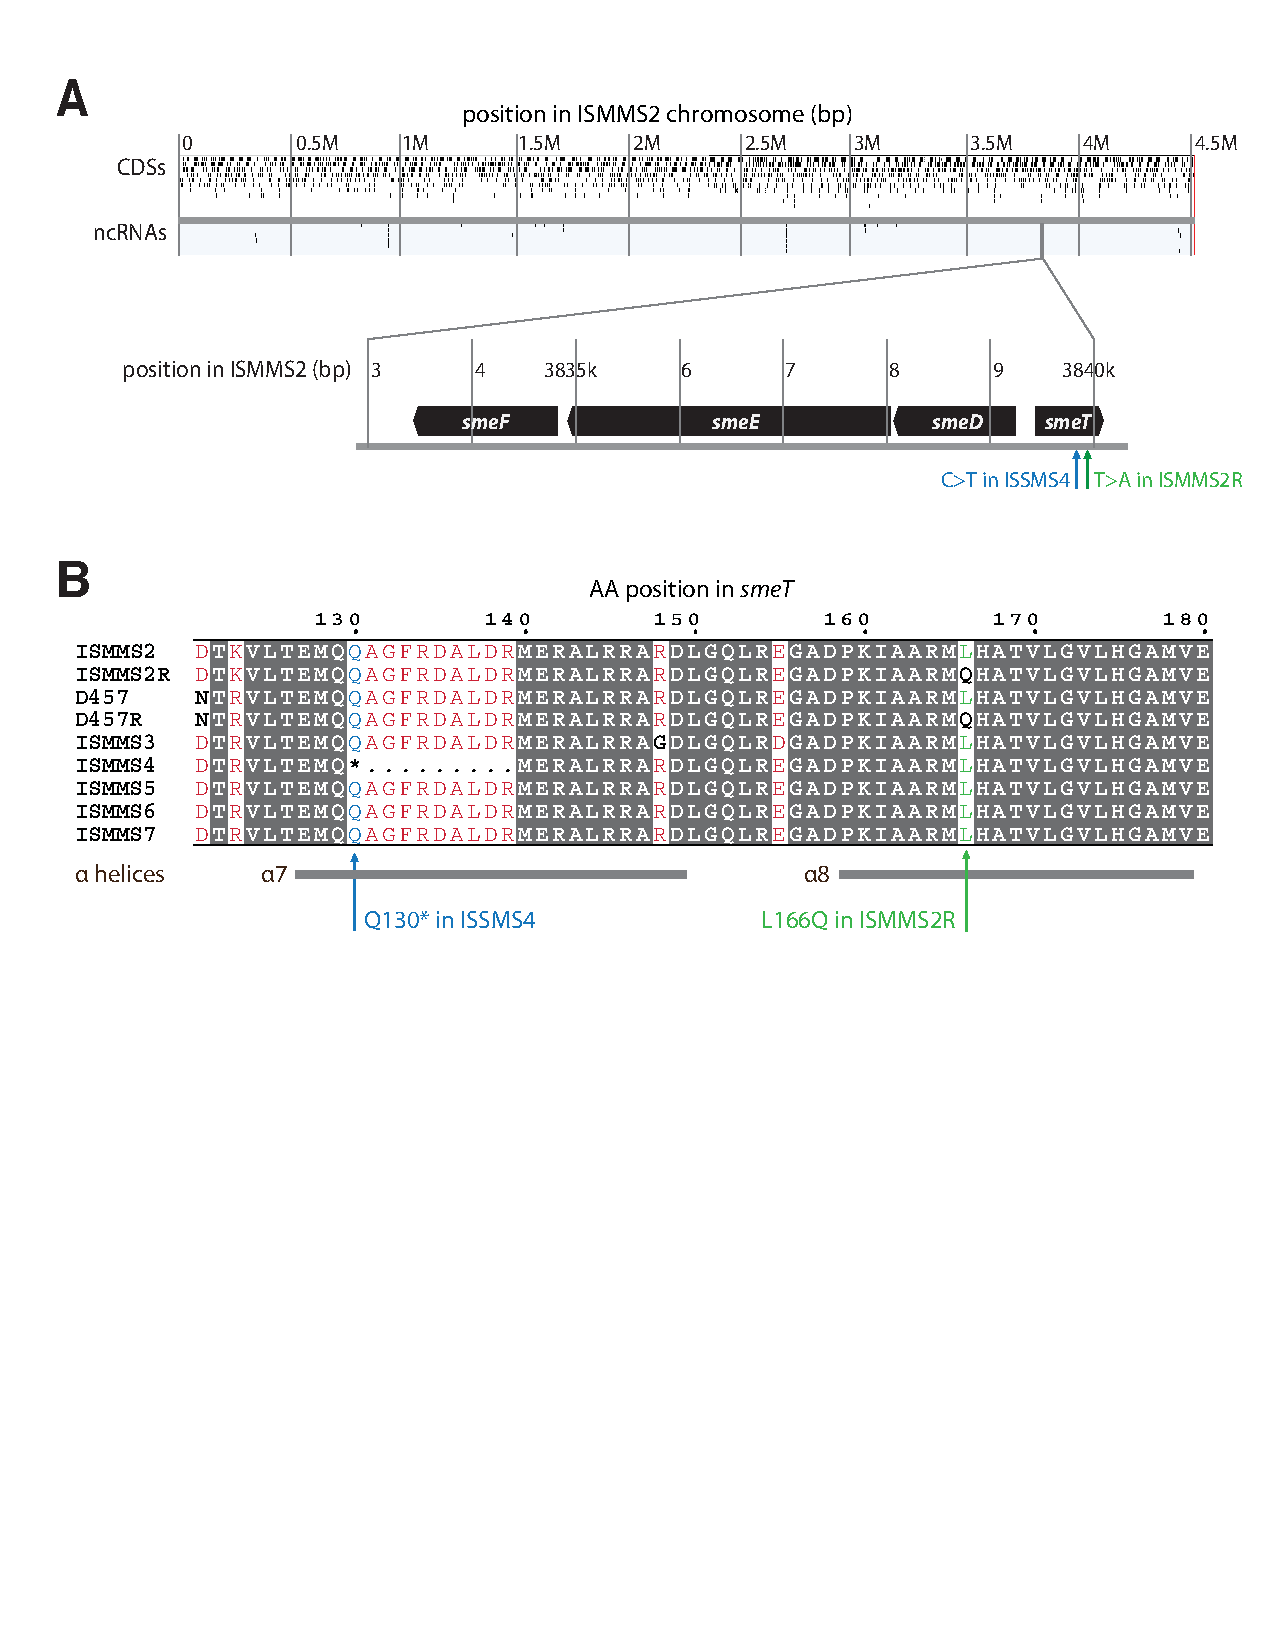
\includegraphics[width=\textwidth]{chap2/snp_location}
  \fullwidthlabelcaption{fig:snp_location}{SNVs observed in quinolone-resistant \emph{S. maltophilia} clinical isolates.}{
    \textbf{Single-nucleotide variants (SNVs) observed in quinolone-resistant \emph{S. maltophilia} clinical isolates.} A, assembled circular chromosome for ISMMS2, including predicted coding domain sequence (CDS) and noncoding RNA (ncRNA) features drawn with ChromoZoom. Horizontal position corresponds to base pair location. The \emph{smeDEF} operon is shown in the detail callout, which highlights both the \emph{smeT} c.497T>A SNV that emerged in ISMMS2R and the aligned location of the \emph{smeT} c.388C>T SNV (encoding a premature stop codon) in ISMMS4. ISMMS2 and ISMMS2R are serial isolates from a single patient before and after development of quinolone resistance, while ISMMS4 was quinolone-resistant at initial isolation from a different patient. B, multiple sequence alignment of part of the predicted \emph{smeT} product in each of the clinical isolates, the D457 reference assembly, and its quinolone resistant counterpart D457R. Predicted α-helices are labeled as grey bars below the sequence. Positions identical in all sequences are shaded with a dark gray background, equivalent substitutions are typeset in red, and non-equivalent substitutions are typeset in boldface black. The L166Q and Q130* (*, stop codon) polymorphisms are highlighted.
  }
\end{figure*}

The same nonsynonymous mutation has been previously observed in an in vitro strain of \emph{S. maltophilia}, D457R, created by selecting single-step tetracycline-resistant mutants from the antibiotic-susceptible clinical strain D457 \autocite{Alonso1997,Sanchez2002}. The mutation is in the eighth α-helix of the \emph{smeT} protein \autocite{Hernandez2009}, which homodimerizes to repress transcription of the \emph{smeDEF} operon \autocite{Hernandez2009,Sanchez2002}. Although the mutation is not in the DNA-binding region, it has been shown to disable the repressor activity of \emph{SmeT},\autocite{Sanchez2002} leading to upregulation of \emph{SmeDEF} and conferring an MDR phenotype \autocite{Alonso2001}.

Figure \ref{fig:snp_location}B shows an amino-acid sequence alignment comparing \emph{SmeT} in D457 and D457R to aligned sequences from our seven isolates. Notably, while none of the remaining isolates shared the same Leu-166→Gln (c.497A>T) mutation, another isolate resistant to levofloxacin, ISMMS4, displayed a C>T mutation at position 388 of \emph{smeT} that creates a premature stop codon that likely disrupts \emph{smeT} function (Figure \ref{fig:snp_location}A and \ref{fig:snp_location}B).

\begin{figure}[htb]
  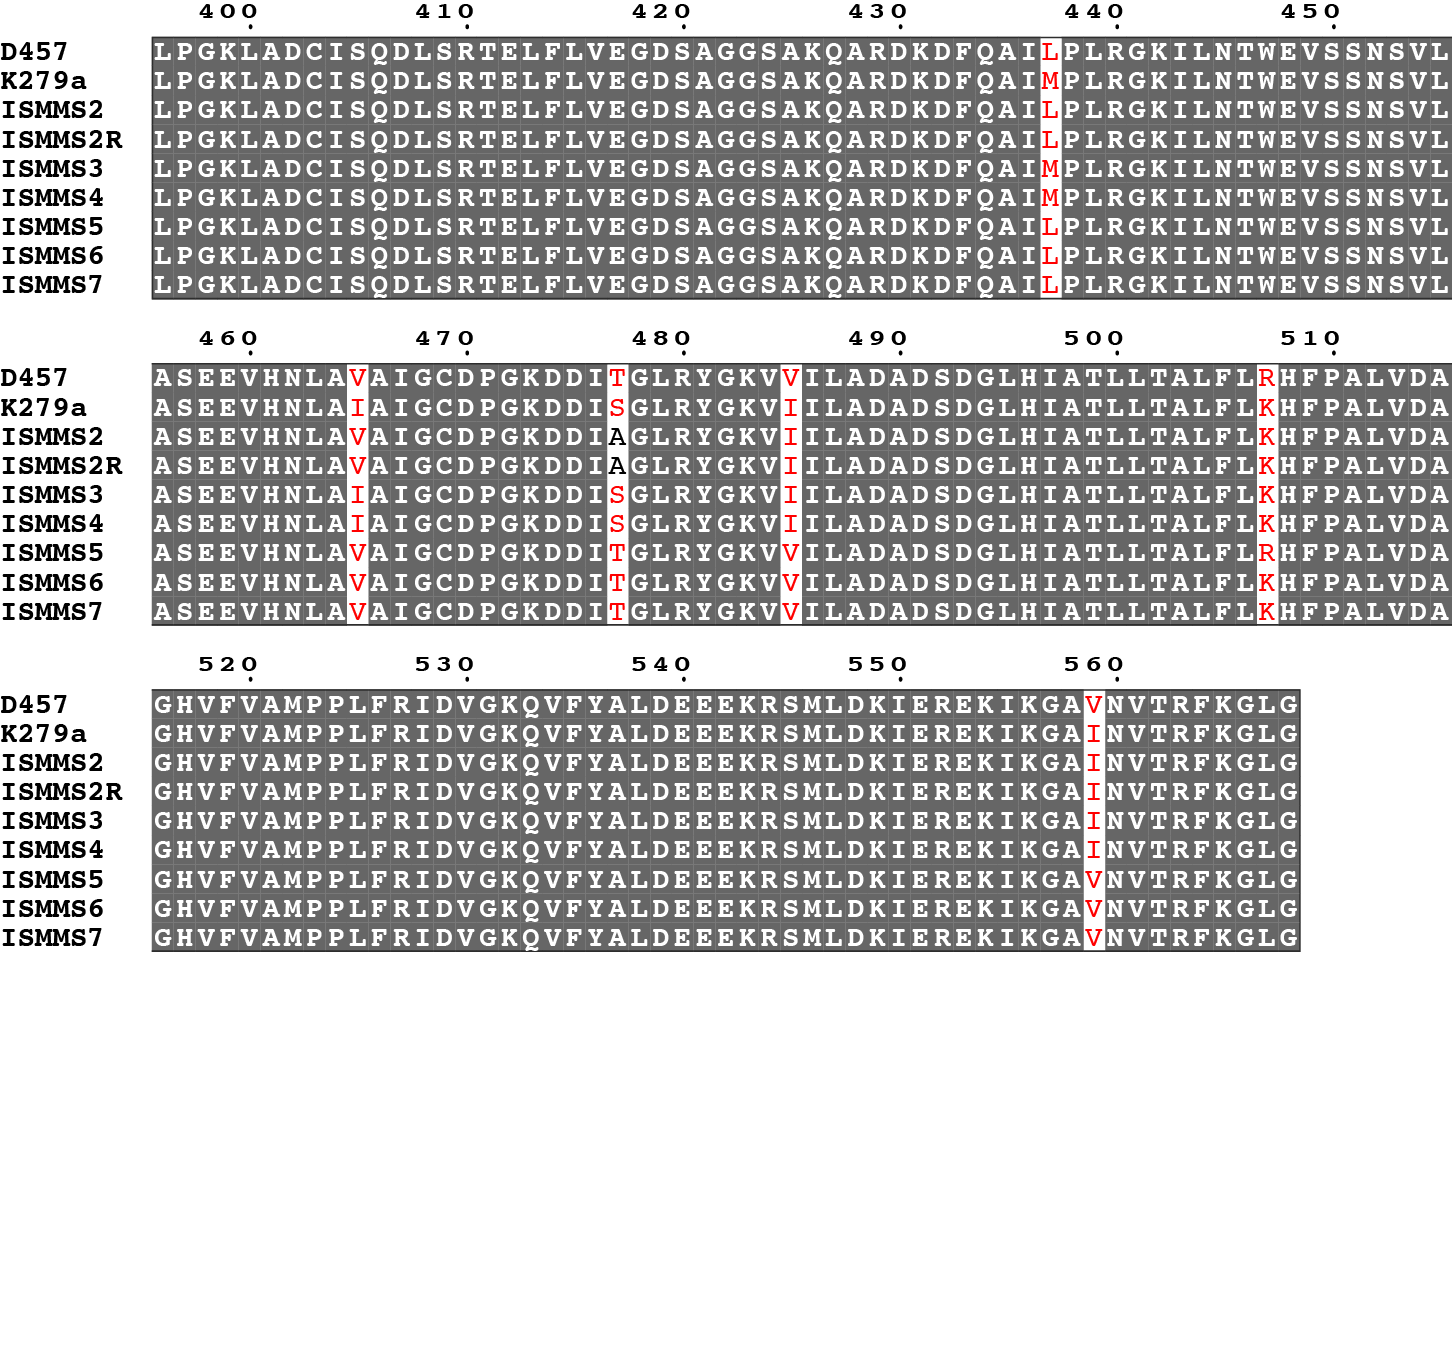
\includegraphics[width=\textwidth]{chap2/qrdr_locus}               
  \caption[Amino-acid sequence alignment for the quinolone-resistance determining region (QRDR) of the \emph{parE} gene]{Amino-acid sequence alignment for the quinolone-resistance determining region (QRDR) of the \emph{parE} gene for seven S. maltophilia clinical isolates (ISMMS2 through 7 and ISMMS2R) and two reference assemblies of clinical isolates obtained from GenBank.}
  \label{fig:qrdr_locus}
\end{figure}
 
The QRDR are loci within genes encoding topoisomerase II and IV subunits known for mutations that confer quinolone resistance in Gram-negative bacteria, although they appear to play a secondary role to efflux systems for resistance emerging during treatment of \emph{S. maltophilia} infection.\autocite{Valdezate2005} An amino-acid sequence alignment of the \emph{gyrA}, \emph{gyrB}, and \emph{parC} genes of our seven isolates and the reference clinical isolates D457 and K279a revealed no differences in the QRDR. Some variants were observed within the QRDR of \emph{parE} (Figure \ref{fig:qrdr_locus}), all of which were consistent with past observations in clinical isolates \autocite{Valdezate2002} except for an Ile-599→Val variant observed in three of our isolates and the D457 reference sequence.

\subsection{Diverse sources of \emph{S. maltophilia} identified with WGS}

Significant genomic diversity was observed among the \emph{S. maltophilia} isolates from all six patients. Figure \ref{fig:steno_phylo} shows a maximum-likelihood phylogeny with branch lengths scaled to SNV distances. Our isolates distribute widely among all four reference assemblies for complete \emph{S. maltophilia} genomes in GenBank. The distances of tens of thousands of SNVs seen in our phylogeny suggest that the natural diversity of pathogenic \emph{S. maltophilia} is greater than that captured by the current set of reference assemblies, even within a single hospital setting. 

\begin{figure}[htb]
  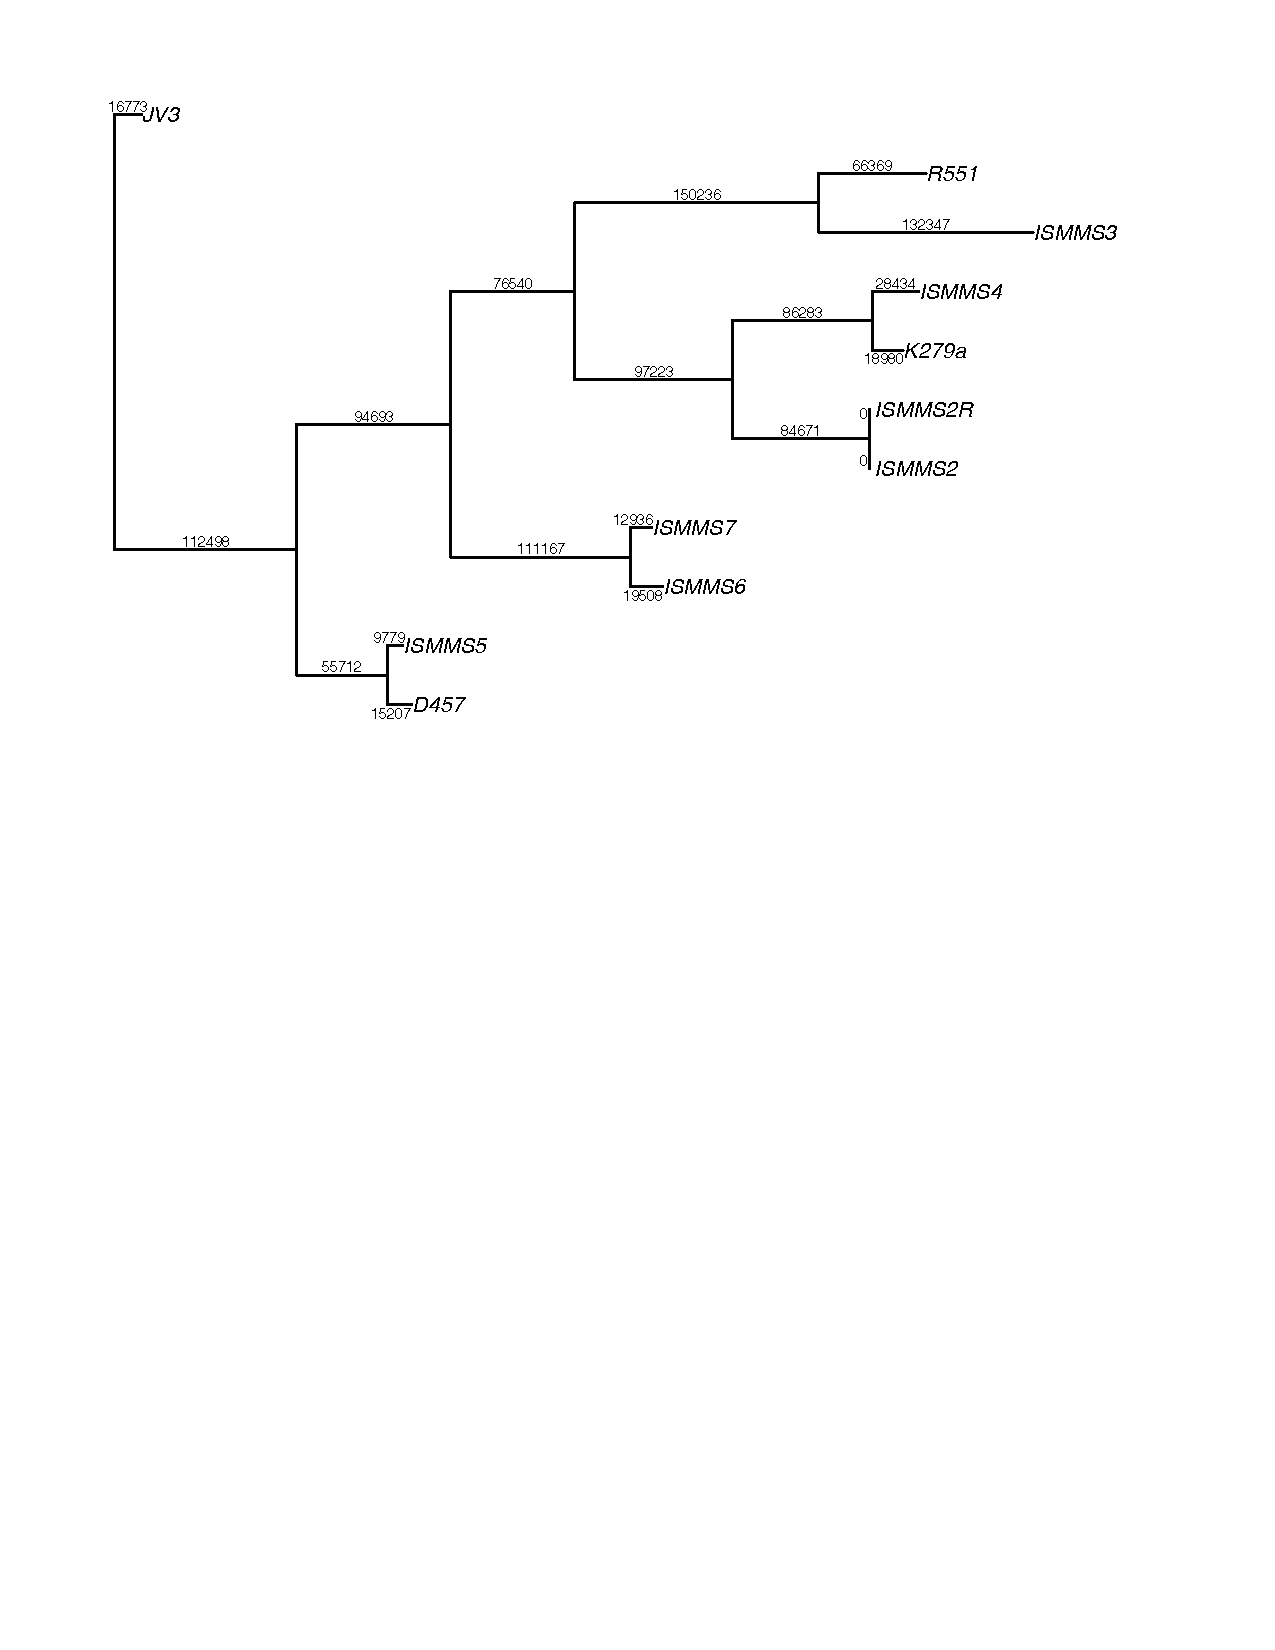
\includegraphics[width=\textwidth]{chap2/phylogram}               
  \caption[Phylogeny of seven \emph{S. maltophilia} clinical isolates]{Phylogeny of seven \emph{S. maltophilia} clinical isolates (ISMMS2 through 7 and ISMMS2R) and four reference assemblies obtained from GenBank. Trees were constructed by inferring ancestral states using RAxML-8.0.2; branch lengths correspond to single-nucleotide polymorphism (SNP) distances from branch points, and are drawn using R version 3.0.3 and the APE library version 3.1-1. The core genome did not contain the \emph{smeT} locus; therefore, the SNV differentiating ISSMS2 and ISMMSR is not observed in this tree.}
  \label{fig:steno_phylo}
\end{figure}

\begin{figure}[htb]
  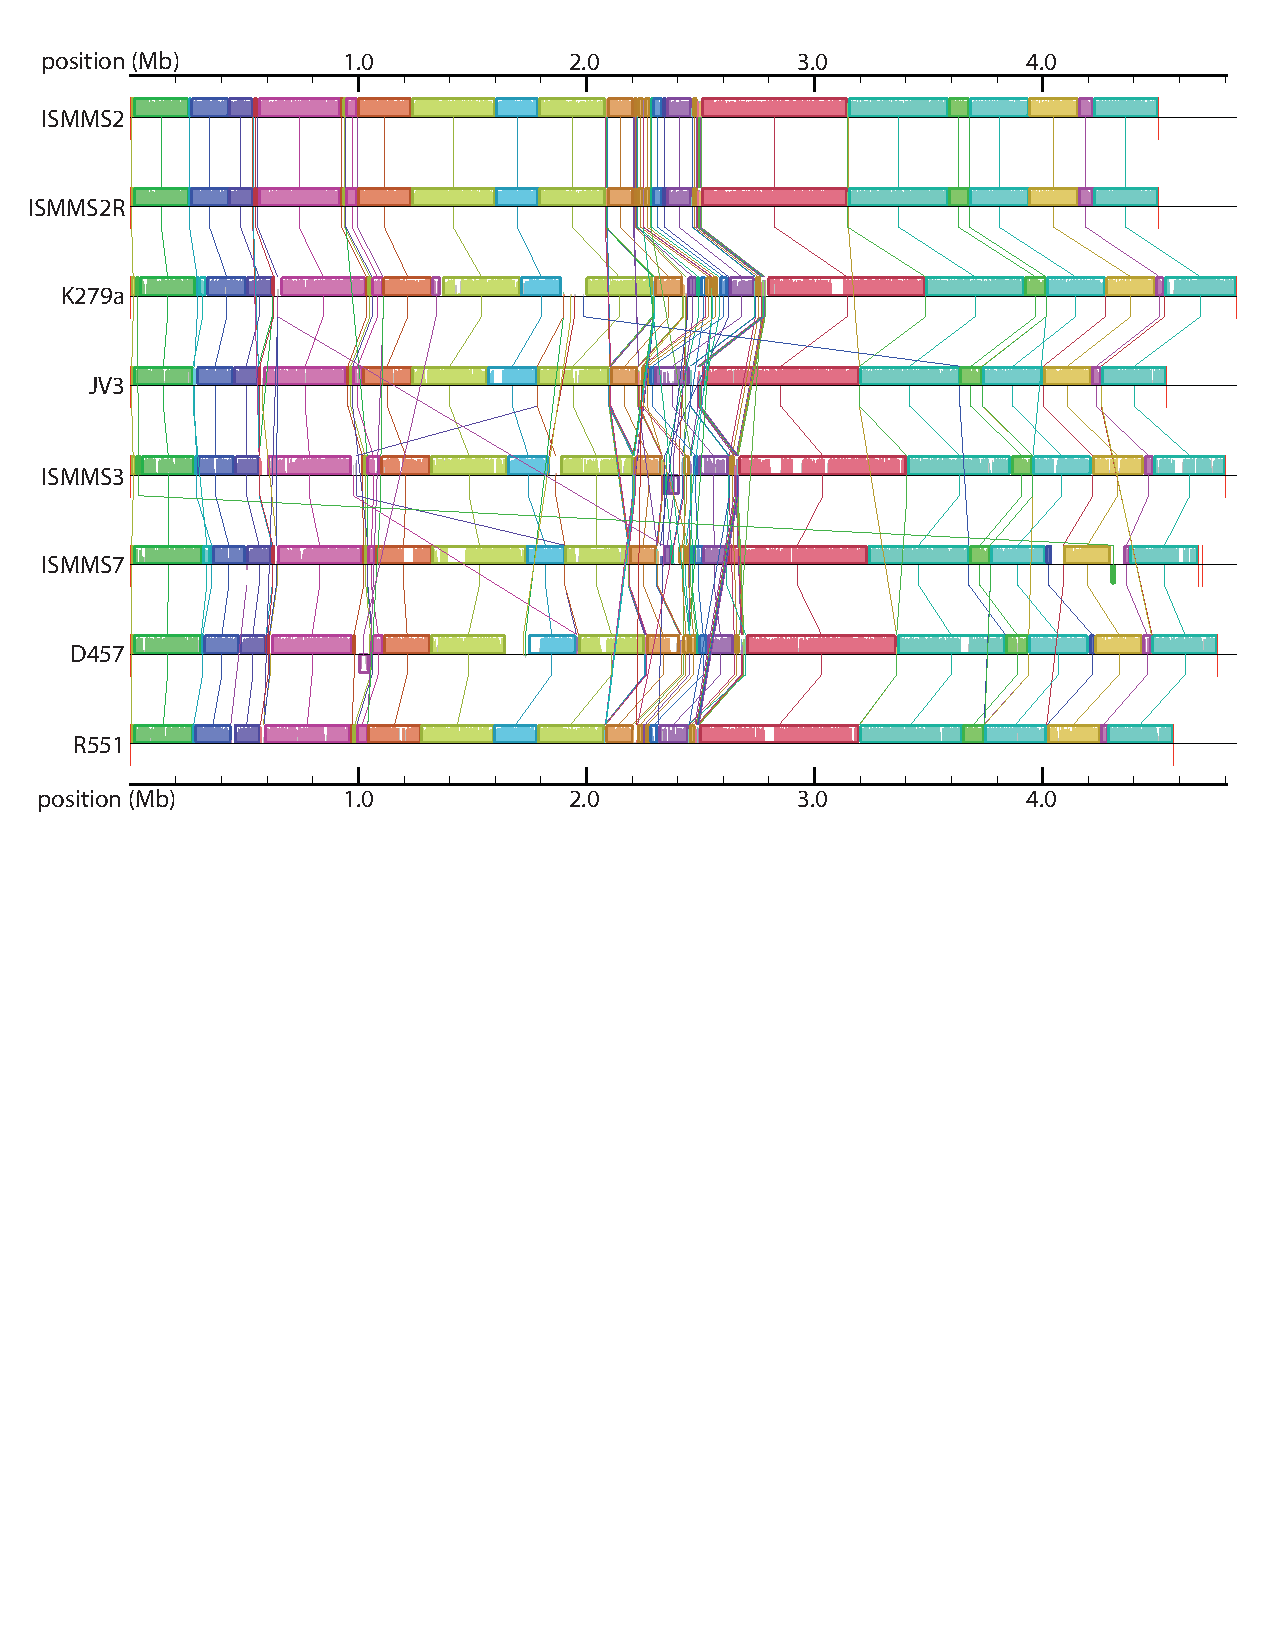
\includegraphics[width=\textwidth]{chap2/mauve_structural_variation}               
  \caption[Genome-scale comparison of four clinical isolates and four reference assemblies]{Genome-scale comparison of four fully assembled \emph{S. maltophilia} clinical isolates and four reference assemblies obtained from GenBank. Mauve 2.4.0 was used to plot locally collinear blocks (LCBs; conserved segments that appear to be internally free from genome rearrangements) as colored rectangles, with gaps representing non-homologous regions. Vertical bars inside each LCB rectangle show the average level of conservation at that region of the genomic sequence. Colored lines connect homologous LCBs among the genomes, and LCBs plotted below the centerline are in the reverse complement orientation relative to the ISMMS2 sequence. At top, sequences for the isolates from before and after development of quinolone resistance (ISSMS2 and ISSMS2R) in the case patient have identical structures.}
  \label{fig:mauve}
\end{figure}

Recombination is not an obvious source of diversity in our \emph{S. maltophilia} isolates. Figure \ref{fig:mauve} depicts whole genome alignments between the four clinical isolates where assembly produced a circularized chromosome and the four GenBank references, showing small areas of non-homology separating large regions of significant homology occurring generally in the same order for each genome. ISMMS2 and ISMMS2R are structurally identical, as expected for serial isolates, while recombination events among other strains are limited to small 1-2kb segments. Epigenetics motif analysis also suggests that the isolates are not related. Table \ref{tab:steno_epimotifs} shows different motifs in isolates from separate patients, implicating differences in type II \& III restriction modification systems between the isolates more likely to be caused by inter-strain/species horizontal transfer of methyltransferases than by intra-strain mutations.\autocite{Srikhanta2010} Together, this demonstrates that transmission did not occur among these six cases and that whole-genome sequencing can comprehensively capture genetic distances and structural variants among diverse clinical isolates of \emph{S. maltophilia}.

\begin{table}[ht]
  \centering
  \begin{tabular}{l l}
    \toprule
    Isolate name & Epigenetic motifs \\
    \midrule
    ISMMS2   & AGT\underline{A}CT \\
    ISMMS2R  & AGT\underline{A}CT \\
    ISMMS3   & None \\
    ISMMS4   & CAG\underline{A}G \\
    ISMMS5   & CTGG\underline{A}C, CACAN\underline{A}G \\
    ISMMS6   & CAAC\underline{A}C, CTG\underline{A}TG, CAACG\underline{A}C \\
    ISMMS7   & CAG\underline{A}G \\
    \bottomrule
  \end{tabular}
  \caption[Epigenetic motifs for clinical isolates of S. maltophilia]{Diverse epigenetic motifs, representing putative target sequences for each strain’s DNA methyltransferase enzymes, discovered for clinical isolates of \emph{S. maltophilia}.  Isolates are named as in Table \ref{tab:steno_pts}. The underlined A’s correspond to putative 6-methyladenine residues, which was the only modification type found in this study.}
  \label{tab:steno_epimotifs}
\end{table}

\section{Discussion}

This is the first report of WGS on serial isolates to characterize the emergence of a resistance mutation in \emph{S. maltophilia} during antibiotic treatment of an active infection. In contrast to studies sequencing highly resistant strains of \emph{S. maltophilia} to reveal various intrinsic and acquired antibiotic resistance genes,\autocite{Crossman2008,Zhao2015} where it remains difficult to assess their relative importance to the phenotype, performing WGS on serial isolates as resistance emerges in vivo allows the causative mutation(s) to be captured. In our patient, the mutation was a SNV that replicates a variant observed in an in vitro model strain created to study the MDR phenotype in 1997.\autocite{Alonso1997} Using WGS and susceptibility testing, we can confirm that this SNV was the only variant to emerge and that it was sufficient to confer quinolone resistance in a clinical case. This underscores the need for clinicians to consider repeating DST during monotherapy if clinical signs suggest therapy failure.

\emph{smeT} appears to play a central role in adaptive resistance to quinolones and other antibiotics effluxed by \emph{smeDEF}, like tetracycline, chloramphenicol, erythromycin, and aminoglycosides. Since any mutation that inactivates this protein would be able to derepress \emph{smeDEF} and confer resistance, \emph{smeT} is under intense selective pressure in the presence of these drugs. In this study, we observed not only a deleterious SNV in the strain that displayed resistance (ISMMS2R), but a premature stop codon in \emph{smeT} in a strain that was already resistant at first isolation (ISMMS4). Certain nucleotide positions appear to be under greater selective pressure than others, as evidenced by our observation of the same mutation that occurred in D457R, and a relative paucity of nonsynonymous coding mutations in \emph{smeT} observed among clinical \emph{smeT} isolates.\autocite{Sanchez2004} Since sustained overexpression of \emph{smeDEF} is physiologically unfavorable \autocite{Alonso2004}, it is possible that pathogenic strains of \emph{S. maltophilia} rely on natural diversity of mutations in the \emph{smeT} locus to activate or deactivate \emph{smeDEF} expression, allowing for rapid adaptation to antibiotic stress, though further study is needed.

Since resistance from a single SNV emerged during a short course of ciprofloxacin, clinicians should be cautioned about using quinolone monotherapy for \emph{S. maltophilia} bacteremia, as highlighted in recent retrospective studies.\autocite{Cho2014a,Wang2014} The wide variety of MDR phenotypes and unreliability of DST results has created uncertainty about appropriate treatment for \emph{S. maltophilia}, but SXT remains the most common choice for monotherapy.\autocite{Brooke2012,Cho2014a,Wang2014} SXT resistance in \emph{S. maltophilia} is not known to be caused by efflux systems but has been linked to Class 1 integrons and ISCR elements.\autocite{Brooke2012} This suggests that spontaneous resistance is less likely to emerge with SXT monotherapy, although a clinical trial comparing the two antibiotics is warranted.\autocite{Cho2014a,Wang2014}

In conclusion, characterizing the full extent of genetic alterations that \emph{S. maltophilia} utilizes to develop antibiotic resistance in vivo and improving genomic surveillance of clinical strains will help refine antibiotic selection criteria available to clinicians. This study furthermore highlights the utility of WGS for profiling the precise mutations underlying emerging antibiotic resistance in clinical cases of bacteremia.

\section*{Notes}

A shortened version of this chapter was published in \textit{Antimicrobial Agents and Chemotherapy}.\autocite{Pak2015a}

\subsection{Funding}

Funding was provided by the Icahn Institute for Genomics and Multiscale Biology at Mount Sinai, and also in part by the NIAID-supported NRSA Institutional Research Training Grant (5 T32 AI 7647-13) for Global Health Research (DRA).

\subsection{Conflict of Interest}

The authors have no conflicts of interest to disclose.

\subsection{Acknowledgements}

We thank Timothy O’Donnell, Tavi Nathanson, Jose Clemente, Flora Samaroo, Angelo Rendo, and members of the clinical microbiology laboratory at Mount Sinai for their contributions. This work was supported in part by the resources and expertise of the Department of Scientific Computing at the Icahn School of Medicine at Mount Sinai.
%% This is an example first chapter.  You should put chapter/appendix that you
%% write into a separate file, and add a line \include{yourfilename} to
%% main.tex, where `yourfilename.tex' is the name of the chapter/appendix file.
%% You can process specific files by typing their names in at the 
%% \files=
%% prompt when you run the file main.tex through LaTeX.

\chapter{Dummy chapter}

\begin{quote}
\textit{In this chapter, I describe my introduction. Lorem ipsum dolor sit amet, consectetur adipiscing elit. Aenean quis dolor bibendum, lobortis mauris a, sollicitudin lacus.}
\end{quote}

\newthought{Lorem ipsum dolor sit amet}, consectetur adipiscing elit. Aenean quis dolor bibendum, lobortis mauris a, sollicitudin lacus. Vivamus sollicitudin orci sed convallis faucibus. Morbi tempor augue vel nunc mollis euismod. Fusce varius fermentum dui, vel ultrices massa fermentum a. \marginnote{Check it out, here's a margin note.}  Pellentesque ac ipsum et libero cursus posuere. Aliquam tincidunt sapien ut ultrices dignissim. Cras tortor leo, pulvinar sagittis lacus et, convallis consectetur quam. Suspendisse potenti. Etiam convallis velit felis, eu rutrum ligula dictum sit amet.

Sed nec suscipit ex. Ut quis urna interdum tortor sollicitudin iaculis. Aliquam purus est, venenatis ac blandit quis, semper quis felis. Integer arcu augue, accumsan at vulputate sed, tristique eu libero.\autocite{Aghaeepour2013} Vivamus ut scelerisque massa. Pellentesque commodo arcu mollis dolor venenatis eleifend. Nulla sit amet rutrum nulla. Nullam leo ante, dapibus vel ipsum quis, bibendum condimentum ligula. Sed faucibus fermentum condimentum. Morbi eu ligula id lacus mattis pharetra. Phasellus auctor est sit amet sapien facilisis molestie vel in ipsum. Etiam malesuada vitae eros sed lacinia.\autocite{Rolph2015} Suspendisse eget iaculis odio, a molestie ex. Mauris ultrices et dolor nec dictum.\autocite{Rolph2015}

Vivamus elementum vehicula orci id mollis.\autocite{Aghaeepour2013,Gelman2006} Duis auctor sapien vel pretium bibendum. Nam aliquam, felis at efficitur pretium, justo libero cursus nisi, sit amet molestie metus massa nec sapien. Donec efficitur porttitor arcu et tempus. Phasellus pretium, diam id suscipit ultrices, lectus odio suscipit risus, at fermentum leo massa vitae eros. Donec elit orci, faucibus et aliquet quis, interdum eget lorem. Nulla a tincidunt odio, vitae commodo metus. Pellentesque bibendum cursus.\autocite{Rolph2015}

\section{Methods}

Aliquam purus est, venenatis ac blandit quis, semper quis felis. Integer arcu augue, accumsan at vulputate sed, tristique eu libero. Vivamus ut scelerisque massa. Pellentesque commodo arcu mollis dolor venenatis eleifend. Nulla sit amet rutrum nulla. Nullam leo ante, dapibus vel ipsum quis, bibendum condimentum ligula. Sed faucibus fermentum condimentum. Morbi eu ligula id lacus mattis pharetra. Phasellus auctor est sit amet sapien facilisis molestie vel in ipsum. Etiam malesuada vitae eros sed lacinia. Suspendisse eget iaculis odio, a molestie ex. Mauris ultrices et dolor nec dictum.

\begin{figure}[htb]
 	\includegraphics[width=\textwidth]{chap1/spin}               
 	 \caption{Check it out, it's a Spin \url{http://spin.media.mit.edu}}
  	\label{fig:spin}
\end{figure}

Phasellus eu nunc eget ante hendrerit porta. Etiam dignissim, mauris vitae luctus sollicitudin, metus purus iaculis tortor, eu lobortis arcu neque vitae ante. Donec egestas nec sem id vulputate. Ut efficitur non massa eget tempor. Nullam rhoncus odio sed dui fringilla semper. Nullam luctus odio felis, ac rutrum mauris maximus sodales. Phasellus non gravida nulla. Aenean congue sapien vitae facilisis luctus. Cum sociis natoque penatibus et magnis dis parturient montes, nascetur ridiculus mus. In laoreet ultrices tellus sed tincidunt. Aenean tempus, dui vel fermentum laoreet, sapien sapien facilisis turpis, vel volutpat sapien libero at mi. Maecenas eleifend libero in enim finibus, eu hendrerit ipsum ornare. Nulla placerat massa eget sapien tincidunt, non venenatis libero accumsan. Nunc ex lectus, rutrum sed varius sed, consectetur vel nisl. Aliquam eu eros vel metus sodales fermentum. Sed quis ultrices nisl, vel semper nibh (Table \ref{tab:sample_table}).

\begin{table}[ht]
  \centering
  \begin{tabular}{l l l l l}
    \toprule
    Column A & Column B & Column C & Column D & Column E \\
    \midrule
    A & B & C & D & E \\
    1 & 2 & 3 & 4 & 5 \\
    10 & 20 & 30 & 40 & 50 \\
    \bottomrule
  \end{tabular}
  \caption{A meaningless table}
  \label{tab:sample_table}
\end{table}

Donec elit orci, faucibus et aliquet quis, interdum eget lorem. Nulla a tincidunt odio, vitae commodo metus.

\subsection{Jiggering the pokery}

\newthought{Sed nec suscipit ex.} Ut quis urna interdum tortor sollicitudin iaculis. Aliquam purus est, venenatis ac blandit quis, semper quis felis. Integer arcu augue, accumsan at vulputate sed, tristique eu libero. Vivamus ut scelerisque massa. Pellentesque commodo arcu mollis dolor venenatis eleifend. Nulla sit amet rutrum nulla. Nullam leo ante, dapibus vel ipsum quis, bibendum condimentum ligula. Sed faucibus fermentum condimentum. Morbi eu ligula id lacus mattis pharetra. Phasellus auctor est sit amet sapien facilisis molestie vel in ipsum. Etiam malesuada vitae eros sed lacinia. Suspendisse eget iaculis odio, a molestie ex. Mauris ultrices et dolor nec dictum.\autocite{Rolph2015,Couderc2015}

Duis auctor sapien vel pretium bibendum. Nam aliquam, felis at efficitur pretium, justo libero cursus nisi, sit amet molestie metus massa nec sapien. Donec efficitur porttitor arcu et tempus. Phasellus pretium, diam id suscipit ultrices, lectus odio suscipit risus, at fermentum leo massa vitae eros. Donec elit orci, faucibus et aliquet quis, interdum eget lorem. Nulla a tincidunt odio, vitae commodo metus. Pellentesque bibendum cursus (Figure \ref{fig:spin_margin}).

Ut quis urna interdum tortor sollicitudin iaculis. Aliquam purus est, venenatis ac blandit quis, semper quis felis. Integer arcu augue, accumsan at vulputate sed, tristique eu libero. Vivamus ut scelerisque massa. Pellentesque commodo arcu mollis dolor venenatis eleifend. Nulla sit amet rutrum nulla. Nullam leo ante, dapibus vel ipsum quis, bibendum condimentum ligula.

\begin{marginfigure}
 	\includegraphics[width=\textwidth]{chap1/spin}  
  \singlespacing             
 	 \caption{Check it out, it's a Spin margin figure \url{http://spin.media.mit.edu}}
  	\label{fig:spin_margin}
\end{marginfigure}


\appendix
\chapter{Appendix Tables}

\begin{quote}
  \emph{I know I've made some very poor decisions recently, but I can give you my complete assurance that my work will be back to normal. I've still got the greatest enthusiasm and confidence in the mission. And I want to help you.}
  \begin{flushright}
    —\smallcaps{HAL}\oldstylenumbers{9000}, \emph{\oldstylenumbers{2001}: A Space Odyssey}
  \end{flushright}
\end{quote}


\vspace{1em}

\begin{quote}
  \emph{\speaker{TARS}: \emph{[as Cooper repairs him]} Settings. General settings. Security settings.}
  
  \emph{\speaker{Cooper}: Honesty, new setting: ninety-five percent.}
  
  \emph{\speaker{TARS}: Confirmed. Additional settings.}
  
  \emph{\speaker{Cooper}: Humor, seventy-five percent.}
  
  \emph{\speaker{TARS}: Confirmed. Self destruct sequence in T minus 10, 9...}
  
  \emph{\speaker{Cooper}: Let's make that sixty percent.}
  
  \emph{\speaker{TARS}: Sixty percent, confirmed. Knock knock.}
  
  \emph{\speaker{Cooper}: You want fifty-five?}
  
  \begin{flushright}
    —\emph{Interstellar}
  \end{flushright}
\end{quote}

% For this appendix, undo tufte-latex's big margin
\newgeometry{left=1in,right=2in,bottom=1.5in,textwidth=5.5in,marginparsep=0pc,marginparwidth=0pc,asymmetric}
% Recalculate fancy header/footer after geometry change (otherwise page numbers are misplaced)
\fancyhfoffset[E,O]{0pt}

\begin{flushleft}
\small

\begin{longtable}[c]{l P{9cm}}
    \toprule
    Variable & Description \\
    \midrule
  \endhead
    \caption[Close correlates for \emph{C. difficile} infection that were excluded from propensity modeling]{\textbf{Variables closely correlated with \emph{Clostridium difficile} infection workup or treatment that were excluded from propensity modeling in Chapter \ref{chap:cdi_cost}.} Raw data for this table are available in tab-separated values format from Figshare at \textsc{doi}:~\href{http://dx.doi.org/10.6084/m9.figshare.4311695}{\texttt{10.6084/m9.figshare.4311695}}. Abbreviation: C.DIFF, \emph{Clostridium difficile}; PCR, polymerase chain reaction; EIA, enzyme immunoassay; CAP, caplet; TAB, tablet; ISO-OSM, iso-osmotic; IV, intravenous; SUSP, suspension}
    \\
    \toprule
    Variable & Description \\
    \midrule
  \endfirsthead
    \midrule
    \multicolumn{2}{r}{\textit{Continued on next page\ldots}} \\
  \endfoot
    \bottomrule
  \endlastfoot
    problem\textunderscore list:008.45 & Intestinal infection due to Clostridium difficile \\
    abnormal\textunderscore labs:4730 & C.DIFF. TOXIN B PCR \\
    abnormal\textunderscore labs:4647 & C.DIFF EIA \\
    abnormal\textunderscore labs:4647 & C.DIFF EIA TOXIN A\&B \\
    meds\textunderscore administered:300025 & VANCOMYCIN ORAL LIQUID REPACKAGE ONLY - 125MG/2.5ML \\
    meds\textunderscore administered:63653  & VANCOMYCIN ORAL \\
    meds\textunderscore administered:8200 & VANCOMYCIN 125 MG CAP \\
    meds\textunderscore administered:14246 & VANCOMYCIN 250 MG/5 ML ORAL SOLUTION \\
    meds\textunderscore administered:300092 & VANCOMYCIN ENEMA \\
    meds\textunderscore administered:13623 & VANCOMYCIN 250 MG CAP \\
    meds\textunderscore administered:5484 & METRONIDAZOLE 250 MG TAB \\
    meds\textunderscore administered:54227 & METRONIDAZOLE ORAL \\
    meds\textunderscore administered:6870 & METRONIDAZOLE 500 MG TAB \\
    meds\textunderscore administered:5484 & METRONIDAZOLE 250 MG TAB \\
    meds\textunderscore administered:6295 & METRONIDAZOLE IN SODIUM CHLORIDE (ISO-OSM) 500 MG/100 ML IV PIGGY BACK \\
    meds\textunderscore administered:400648 & METRONIDAZOLE 250 MG/50 ML ISO-OSMOTIC SOLUTION \\
    meds\textunderscore administered:1527 & METRONIDAZOLE HCL 500 MG IV SOLUTION \\
    meds\textunderscore administered:19702 & METRONIDAZOLE 375 MG CAP \\
    meds\textunderscore administered:300009 & METRONIDAZOLE 50 MG/ML ORAL SUSP \\
    meds\textunderscore administered:400660 & METRONIDAZOLE 750 MG/150 ML ISO-OSMOTIC SOLUTION \\
    meds\textunderscore reported:300025 & VANCOMYCIN ORAL LIQUID REPACKAGE ONLY - 125MG/2.5ML \\
    meds\textunderscore administered:14246 & VANCOMYCIN 250 MG/5 ML ORAL SOLUTION \\
    meds\textunderscore administered:300092 & VANCOMYCIN ENEMA \\
    meds\textunderscore administered:13623 & VANCOMYCIN 250 MG CAP \\
    meds\textunderscore administered:5484 & METRONIDAZOLE 250 MG TAB \\
    meds\textunderscore administered:54227 & METRONIDAZOLE ORAL \\
    meds\textunderscore administered:6870 & METRONIDAZOLE 500 MG TAB \\
    meds\textunderscore administered:5484 & METRONIDAZOLE 250 MG TAB \\
    meds\textunderscore administered:6295 & METRONIDAZOLE IN SODIUM CHLORIDE (ISO-OSM) 500 MG/100 ML IV PIGGY BACK \\
    meds\textunderscore administered:400648 & METRONIDAZOLE 250 MG/50 ML ISO-OSMOTIC SOLUTION \\
    meds\textunderscore administered:1527 & METRONIDAZOLE HCL 500 MG IV SOLUTION \\
    meds\textunderscore administered:19702 & METRONIDAZOLE 375 MG CAP \\
    meds\textunderscore administered:300009 & METRONIDAZOLE 50 MG/ML ORAL SUSP \\
    meds\textunderscore administered:400660 & METRONIDAZOLE 750 MG/150 ML ISO-OSMOTIC SOLUTION \\
    meds\textunderscore reported:300025 & VANCOMYCIN ORAL LIQUID REPACKAGE ONLY - 125MG/2.5ML \\
    meds\textunderscore reported:63653  & VANCOMYCIN ORAL \\
    meds\textunderscore reported:8200 & VANCOMYCIN 125 MG CAP \\
    meds\textunderscore reported:14246 & VANCOMYCIN 250 MG/5 ML ORAL SOLUTION \\
    meds\textunderscore reported:300092 & VANCOMYCIN ENEMA \\
    meds\textunderscore reported:13623 & VANCOMYCIN 250 MG CAP \\
    meds\textunderscore reported:5484 & METRONIDAZOLE 250 MG TAB \\
    meds\textunderscore reported:54227 & METRONIDAZOLE ORAL \\
    meds\textunderscore reported:6870 & METRONIDAZOLE 500 MG TAB \\
    meds\textunderscore reported:5484 & METRONIDAZOLE 250 MG TAB \\
    meds\textunderscore reported:6295 & METRONIDAZOLE IN SODIUM CHLORIDE (ISO-OSM) 500 MG/100 ML IV PIGGY BACK \\
    meds\textunderscore reported:400648 & METRONIDAZOLE 250 MG/50 ML ISO-OSMOTIC SOLUTION \\
    meds\textunderscore reported:1527 & METRONIDAZOLE HCL 500 MG IV SOLUTION \\
    meds\textunderscore reported:19702 & METRONIDAZOLE 375 MG CAP \\
    meds\textunderscore reported:300009 & METRONIDAZOLE 50 MG/ML ORAL SUSP \\
    meds\textunderscore reported:400660 & METRONIDAZOLE 750 MG/150 ML ISO-OSMOTIC SOLUTION \\
    problem\textunderscore list:041.84 & Other specified bacterial infections in conditions classified elsewhere and of unspecified site, other anaerobes \\
    problem\textunderscore list:V07.0 & Need for isolation \\
    problem\textunderscore list:V02.3 & Carrier or suspected carrier of other gastrointestinal pathogens \\
    problem\textunderscore list:787.91 & Diarrhea
    \label{tab:excluded_vars}
\end{longtable}

\newpage

\begin{longtable}[c]{l l l l}
    \toprule
    Isotope & Target & Clone & Source \\
    \midrule
  \endhead
    \caption[Antibodies used for CyTOF analysis in Chapter \ref{chap:chik}]{
      \textbf{Antibodies used for CyTOF analysis in Chapter \ref{chap:chik}}. All antibodies were either purchased directly from Fluidigm or conjugated in-house using X8 conjugation kits. 
    }
    \\
    \toprule
    Isotope & Target & Clone & Source \\
    \midrule
  \endfirsthead
    \midrule
    \multicolumn{2}{r}{\textit{Continued on next page\ldots}} \\
  \endfoot
    \bottomrule
  \endlastfoot
    113 In & CD57 & HCD57 & Biolegend \\
    115 In & CD45 & HI130 & Biolegend \\
    142 Nd & CD19 & HIB19 & Biolegend \\
    143 Nd & CD45RA & HI100 & Biolegend \\
    144 Nd & CD141 & M80 & Biolegend \\
    145 Nd & CD4 & RPA-T4 & Biolegend \\
    146 Nd & CD8 & RPA-T8 & Biolegend \\
    147 Sm & CD20 & 2H7 & Fluidigm \\
    148 Nd & CD16 & 3G8 & Biolegend \\
    149 Sm & CD127 & A019D5 & Biolegend \\
    150 Nd & CD1c & L161 & Biolegend \\
    151 Eu & CD123 & 6H6 & Biolegend \\
    152 Sm & CD66b & G10F5 & Biolegend \\
    153 Eu & CXCR5 & RF8B2 & Fluidigm \\
    154 Sm & CD86 & IT2.2 & Biolegend \\
    155 Gd & CD27 & O323 & Biolegend \\
    156 Gd & CCR5 & NP-6G4 & Fluidigm \\
    158 Gd & CHIKV & CHK-152 & Biomatik \\
    159 Tb & CD11c & Bu15 & Fluidigm \\
    160 Gd & CD14 & M5E2 & Biolegend \\
    161 Dy & CD56 & B159 & BD Biosciences \\
    162 Dy & CD80 & 2D10.4 & Fluidigm \\
    163 Dy & CCR4 & 205410 & R\&D Systems \\
    164 Dy & CD40 & 5C3 & Biolegend \\
    165 Ho & CCR6 & G034E3 & Biolegend \\
    166 Er & CD25 & M-A251 & Biolegend \\
    167 Er & CCR7 & G043H7 & Biolegend \\
    168 Er & CD3 & UCHT1 & Biolegend \\
    169 Tm & CX3CR1 & 2A9-1 & Biolegend \\
    170 Er & CD38 & HB-7 & Biolegend \\
    171 Yb & CD161 & HP-3G10 & Biolegend \\
    172 Yb & CD209 & 9E9A8 & Biolegend \\
    173 Yb & CXCR3 & G025H7 & Biolegend \\
    174 Yb & HLADR & L243 & Biolegend \\
    175 Lu & PD-1 & EH12.2H7 & Fluidigm \\
    176 Yb & CD54 & HCD54 & Biolegend \\
    209 Bi & CD11b & ICRF44 & Fluidigm \\
    194Pt & CD45 (acute BC) & HI130 & Biolegend \\
    198Pt  & CD45 (conv BC) & HI130 & Biolegend \\
    103 Rh  & Viability & n/a & Fluidigm \\
    191/193 Ir & DNA & n/a & Fluidigm
    \label{tab:chik_antibodies}
\end{longtable}

\end{flushleft}

% Restore the geometry of tufte-latex's big right margin
\restoregeometry
% Restore tufte-latex's fancy header/footer offsets
\tuftefancyhfoffset

\clearpage
\newpage

% Recalculate fancy header/footer after geometry change (otherwise page numbers are misplaced)
%\fancyhfoffset[E,O]{0pt}

%% Prints the bibliography chapter. Note that this is a biblatex macro, *not* natbib.
\begin{singlespace}

\printbibliography[heading=bibintoc]

\end{singlespace}


\end{document}